% ****** Start of file apssamp.tex ******
%
%   This file is part of the APS files in the REVTeX 4.1 distribution.
%   Version 4.1r of REVTeX, August 2010
%
%   Copyright (c) 2009, 2010 The American Physical Society.
%
%   See the REVTeX 4 README file for restrictions and more information.
%
% TeX'ing this file requires that you have AMS-LaTeX 2.0 installed
% as well as the rest of the prerequisites for REVTeX 4.1
%
% See the REVTeX 4 README file
% It also requires running BibTeX. The commands are as follows:
%
%  1)  latex apssamp.tex
%  2)  bibtex apssamp
%  3)  latex apssamp.tex
%  4)  latex apssamp.tex
%
\documentclass[%
 reprint,	
%superscriptaddress,
%groupedaddress,
%unsortedaddress,
%runinaddress,
%frontmatterverbose, 
%preprint,
showpacs,
% preprintnumbers,
%nofootinbib,
%nobibnotes,
%bibnotes,
 amsmath,amssymb,
 aps,
 superscriptaddress,
%prl,
%prc,
%prb,
%rmp,
%prstab,
%prstper,
%floatfix,
]{revtex4-1}

\usepackage{graphicx}% Include figure files
\usepackage{dcolumn}% Align table columns on decimal point
\usepackage{bm}% bold math
\usepackage{url}
\usepackage{lipsum}
\usepackage{color}
\usepackage{hyperref}% add hypertext capabilities
\usepackage[mathlines]{lineno}% Enable numbering of text and display math
\usepackage{upgreek}
\usepackage{biolinum}
\linenumbers\relax % Commence numbering lines

%\usepackage[showframe,%Uncomment any one of the following lines to test 
%%scale=0.7, marginratio={1:1, 2:3}, ignoreall,% default settings
%%text={7in,10in},centering,
%%margin=1.5in,
%%total={6.5in,8.75in}, top=1.2in, left=0.9in, includefoot,
%%height=10in,a5paper,hmargin={3cm,0.8in},
%]{geometry}

% \setcounter{secnumdepth}{5}
\begin{document}

\preprint{APS/123-QED}

\title{Probing Strangeness Canonical Ensemble with $K^{-}$, $\phi(1020)$ and $\Xi^{-}$ Production in Au+Au Collisions at ${\sqrt{s_{\rm NN}} = \rm{3\,GeV}}$}% Force line breaks with \\
%\thanks{A footnote to the article title}%

% \author{Ann Author}
% \altaffiliation[Also at ]{Physics Department, XYZ University.}%Lines break automatically or can be forced with \\
% \author{Second Author}%
% \email{Second.Author@institution.edu}
% \affiliation{% Authors' institution and/or address\\ This line break forced with \textbackslash\textbackslash
% }%
\affiliation{Abilene Christian University, Abilene, Texas   79699}
\affiliation{AGH University of Science and Technology, FPACS, Cracow 30-059, Poland}
\affiliation{Alikhanov Institute for Theoretical and Experimental Physics NRC "Kurchatov Institute", Moscow 117218}
\affiliation{Argonne National Laboratory, Argonne, Illinois 60439}
\affiliation{American University of Cairo, New Cairo 11835, New Cairo, Egypt}
\affiliation{Brookhaven National Laboratory, Upton, New York 11973}
\affiliation{University of California, Berkeley, California 94720}
\affiliation{University of California, Davis, California 95616}
\affiliation{University of California, Los Angeles, California 90095}
\affiliation{University of California, Riverside, California 92521}
\affiliation{Central China Normal University, Wuhan, Hubei 430079 }
\affiliation{University of Illinois at Chicago, Chicago, Illinois 60607}
\affiliation{Creighton University, Omaha, Nebraska 68178}
\affiliation{Czech Technical University in Prague, FNSPE, Prague 115 19, Czech Republic}
\affiliation{Technische Universit\"at Darmstadt, Darmstadt 64289, Germany}
\affiliation{ELTE E\"otv\"os Lor\'and University, Budapest, Hungary H-1117}
\affiliation{Frankfurt Institute for Advanced Studies FIAS, Frankfurt 60438, Germany}
\affiliation{Fudan University, Shanghai, 200433 }
\affiliation{University of Heidelberg, Heidelberg 69120, Germany }
\affiliation{University of Houston, Houston, Texas 77204}
\affiliation{Huzhou University, Huzhou, Zhejiang  313000}
\affiliation{Indian Institute of Science Education and Research (IISER), Berhampur 760010 , India}
\affiliation{Indian Institute of Science Education and Research (IISER) Tirupati, Tirupati 517507, India}
\affiliation{Indian Institute Technology, Patna, Bihar 801106, India}
\affiliation{Indiana University, Bloomington, Indiana 47408}
\affiliation{Institute of Modern Physics, Chinese Academy of Sciences, Lanzhou, Gansu 730000 }
\affiliation{University of Jammu, Jammu 180001, India}
\affiliation{Joint Institute for Nuclear Research, Dubna 141 980}
\affiliation{Kent State University, Kent, Ohio 44242}
\affiliation{University of Kentucky, Lexington, Kentucky 40506-0055}
\affiliation{Lawrence Berkeley National Laboratory, Berkeley, California 94720}
\affiliation{Lehigh University, Bethlehem, Pennsylvania 18015}
\affiliation{Max-Planck-Institut f\"ur Physik, Munich 80805, Germany}
\affiliation{Michigan State University, East Lansing, Michigan 48824}
\affiliation{National Research Nuclear University MEPhI, Moscow 115409}
\affiliation{National Institute of Science Education and Research, HBNI, Jatni 752050, India}
\affiliation{National Cheng Kung University, Tainan 70101 }
\affiliation{Nuclear Physics Institute of the CAS, Rez 250 68, Czech Republic}
\affiliation{Ohio State University, Columbus, Ohio 43210}
\affiliation{Institute of Nuclear Physics PAN, Cracow 31-342, Poland}
\affiliation{Panjab University, Chandigarh 160014, India}
\affiliation{Pennsylvania State University, University Park, Pennsylvania 16802}
\affiliation{NRC "Kurchatov Institute", Institute of High Energy Physics, Protvino 142281}
\affiliation{Purdue University, West Lafayette, Indiana 47907}
\affiliation{Rice University, Houston, Texas 77251}
\affiliation{Rutgers University, Piscataway, New Jersey 08854}
\affiliation{Universidade de S\~ao Paulo, S\~ao Paulo, Brazil 05314-970}
\affiliation{University of Science and Technology of China, Hefei, Anhui 230026}
\affiliation{Shandong University, Qingdao, Shandong 266237}
\affiliation{Shanghai Institute of Applied Physics, Chinese Academy of Sciences, Shanghai 201800}
\affiliation{Southern Connecticut State University, New Haven, Connecticut 06515}
\affiliation{State University of New York, Stony Brook, New York 11794}
\affiliation{Instituto de Alta Investigaci\'on, Universidad de Tarapac\'a, Arica 1000000, Chile}
\affiliation{Temple University, Philadelphia, Pennsylvania 19122}
\affiliation{Texas A\&M University, College Station, Texas 77843}
\affiliation{University of Texas, Austin, Texas 78712}
\affiliation{Tsinghua University, Beijing 100084}
\affiliation{University of Tsukuba, Tsukuba, Ibaraki 305-8571, Japan}
\affiliation{Valparaiso University, Valparaiso, Indiana 46383}
\affiliation{Variable Energy Cyclotron Centre, Kolkata 700064, India}
\affiliation{Warsaw University of Technology, Warsaw 00-661, Poland}
\affiliation{Wayne State University, Detroit, Michigan 48201}
\affiliation{Yale University, New Haven, Connecticut 06520}

\author{M.~S.~Abdallah}\affiliation{American University of Cairo, New Cairo 11835, New Cairo, Egypt}
\author{B.~E.~Aboona}\affiliation{Texas A\&M University, College Station, Texas 77843}
\author{J.~Adam}\affiliation{Brookhaven National Laboratory, Upton, New York 11973}
\author{L.~Adamczyk}\affiliation{AGH University of Science and Technology, FPACS, Cracow 30-059, Poland}
\author{J.~R.~Adams}\affiliation{Ohio State University, Columbus, Ohio 43210}
\author{J.~K.~Adkins}\affiliation{University of Kentucky, Lexington, Kentucky 40506-0055}
\author{G.~Agakishiev}\affiliation{Joint Institute for Nuclear Research, Dubna 141 980}
\author{I.~Aggarwal}\affiliation{Panjab University, Chandigarh 160014, India}
\author{M.~M.~Aggarwal}\affiliation{Panjab University, Chandigarh 160014, India}
\author{Z.~Ahammed}\affiliation{Variable Energy Cyclotron Centre, Kolkata 700064, India}
\author{I.~Alekseev}\affiliation{Alikhanov Institute for Theoretical and Experimental Physics NRC "Kurchatov Institute", Moscow 117218}\affiliation{National Research Nuclear University MEPhI, Moscow 115409}
\author{D.~M.~Anderson}\affiliation{Texas A\&M University, College Station, Texas 77843}
\author{A.~Aparin}\affiliation{Joint Institute for Nuclear Research, Dubna 141 980}
\author{E.~C.~Aschenauer}\affiliation{Brookhaven National Laboratory, Upton, New York 11973}
\author{M.~U.~Ashraf}\affiliation{Central China Normal University, Wuhan, Hubei 430079 }
\author{F.~G.~Atetalla}\affiliation{Kent State University, Kent, Ohio 44242}
\author{A.~Attri}\affiliation{Panjab University, Chandigarh 160014, India}
\author{G.~S.~Averichev}\affiliation{Joint Institute for Nuclear Research, Dubna 141 980}
\author{V.~Bairathi}\affiliation{Instituto de Alta Investigaci\'on, Universidad de Tarapac\'a, Arica 1000000, Chile}
\author{W.~Baker}\affiliation{University of California, Riverside, California 92521}
\author{J.~G.~Ball~Cap}\affiliation{University of Houston, Houston, Texas 77204}
\author{K.~Barish}\affiliation{University of California, Riverside, California 92521}
\author{A.~Behera}\affiliation{State University of New York, Stony Brook, New York 11794}
\author{R.~Bellwied}\affiliation{University of Houston, Houston, Texas 77204}
\author{P.~Bhagat}\affiliation{University of Jammu, Jammu 180001, India}
\author{A.~Bhasin}\affiliation{University of Jammu, Jammu 180001, India}
\author{J.~Bielcik}\affiliation{Czech Technical University in Prague, FNSPE, Prague 115 19, Czech Republic}
\author{J.~Bielcikova}\affiliation{Nuclear Physics Institute of the CAS, Rez 250 68, Czech Republic}
\author{I.~G.~Bordyuzhin}\affiliation{Alikhanov Institute for Theoretical and Experimental Physics NRC "Kurchatov Institute", Moscow 117218}
\author{J.~D.~Brandenburg}\affiliation{Brookhaven National Laboratory, Upton, New York 11973}
\author{A.~V.~Brandin}\affiliation{National Research Nuclear University MEPhI, Moscow 115409}
\author{I.~Bunzarov}\affiliation{Joint Institute for Nuclear Research, Dubna 141 980}
\author{J.~Butterworth}\affiliation{Rice University, Houston, Texas 77251}
\author{X.~Z.~Cai}\affiliation{Shanghai Institute of Applied Physics, Chinese Academy of Sciences, Shanghai 201800}
\author{H.~Caines}\affiliation{Yale University, New Haven, Connecticut 06520}
\author{M.~Calder{\'o}n~de~la~Barca~S{\'a}nchez}\affiliation{University of California, Davis, California 95616}
\author{D.~Cebra}\affiliation{University of California, Davis, California 95616}
\author{I.~Chakaberia}\affiliation{Lawrence Berkeley National Laboratory, Berkeley, California 94720}\affiliation{Brookhaven National Laboratory, Upton, New York 11973}
\author{P.~Chaloupka}\affiliation{Czech Technical University in Prague, FNSPE, Prague 115 19, Czech Republic}
\author{B.~K.~Chan}\affiliation{University of California, Los Angeles, California 90095}
\author{F-H.~Chang}\affiliation{National Cheng Kung University, Tainan 70101 }
\author{Z.~Chang}\affiliation{Brookhaven National Laboratory, Upton, New York 11973}
\author{N.~Chankova-Bunzarova}\affiliation{Joint Institute for Nuclear Research, Dubna 141 980}
\author{A.~Chatterjee}\affiliation{Central China Normal University, Wuhan, Hubei 430079 }
\author{S.~Chattopadhyay}\affiliation{Variable Energy Cyclotron Centre, Kolkata 700064, India}
\author{D.~Chen}\affiliation{University of California, Riverside, California 92521}
\author{J.~Chen}\affiliation{Shandong University, Qingdao, Shandong 266237}
\author{J.~H.~Chen}\affiliation{Fudan University, Shanghai, 200433 }
\author{X.~Chen}\affiliation{University of Science and Technology of China, Hefei, Anhui 230026}
\author{Z.~Chen}\affiliation{Shandong University, Qingdao, Shandong 266237}
\author{J.~Cheng}\affiliation{Tsinghua University, Beijing 100084}
\author{M.~Chevalier}\affiliation{University of California, Riverside, California 92521}
\author{S.~Choudhury}\affiliation{Fudan University, Shanghai, 200433 }
\author{W.~Christie}\affiliation{Brookhaven National Laboratory, Upton, New York 11973}
\author{X.~Chu}\affiliation{Brookhaven National Laboratory, Upton, New York 11973}
\author{H.~J.~Crawford}\affiliation{University of California, Berkeley, California 94720}
\author{M.~Csan\'{a}d}\affiliation{ELTE E\"otv\"os Lor\'and University, Budapest, Hungary H-1117}
\author{M.~Daugherity}\affiliation{Abilene Christian University, Abilene, Texas   79699}
\author{T.~G.~Dedovich}\affiliation{Joint Institute for Nuclear Research, Dubna 141 980}
\author{I.~M.~Deppner}\affiliation{University of Heidelberg, Heidelberg 69120, Germany }
\author{A.~A.~Derevschikov}\affiliation{NRC "Kurchatov Institute", Institute of High Energy Physics, Protvino 142281}
\author{A.~Dhamija}\affiliation{Panjab University, Chandigarh 160014, India}
\author{L.~Di~Carlo}\affiliation{Wayne State University, Detroit, Michigan 48201}
\author{L.~Didenko}\affiliation{Brookhaven National Laboratory, Upton, New York 11973}
\author{P.~Dixit}\affiliation{Indian Institute of Science Education and Research (IISER), Berhampur 760010 , India}
\author{X.~Dong}\affiliation{Lawrence Berkeley National Laboratory, Berkeley, California 94720}
\author{J.~L.~Drachenberg}\affiliation{Abilene Christian University, Abilene, Texas   79699}
\author{E.~Duckworth}\affiliation{Kent State University, Kent, Ohio 44242}
\author{J.~C.~Dunlop}\affiliation{Brookhaven National Laboratory, Upton, New York 11973}
\author{N.~Elsey}\affiliation{Wayne State University, Detroit, Michigan 48201}
\author{J.~Engelage}\affiliation{University of California, Berkeley, California 94720}
\author{G.~Eppley}\affiliation{Rice University, Houston, Texas 77251}
\author{S.~Esumi}\affiliation{University of Tsukuba, Tsukuba, Ibaraki 305-8571, Japan}
\author{O.~Evdokimov}\affiliation{University of Illinois at Chicago, Chicago, Illinois 60607}
\author{A.~Ewigleben}\affiliation{Lehigh University, Bethlehem, Pennsylvania 18015}
\author{O.~Eyser}\affiliation{Brookhaven National Laboratory, Upton, New York 11973}
\author{R.~Fatemi}\affiliation{University of Kentucky, Lexington, Kentucky 40506-0055}
\author{F.~M.~Fawzi}\affiliation{American University of Cairo, New Cairo 11835, New Cairo, Egypt}
\author{S.~Fazio}\affiliation{Brookhaven National Laboratory, Upton, New York 11973}
\author{P.~Federic}\affiliation{Nuclear Physics Institute of the CAS, Rez 250 68, Czech Republic}
\author{J.~Fedorisin}\affiliation{Joint Institute for Nuclear Research, Dubna 141 980}
\author{C.~J.~Feng}\affiliation{National Cheng Kung University, Tainan 70101 }
\author{Y.~Feng}\affiliation{Purdue University, West Lafayette, Indiana 47907}
\author{P.~Filip}\affiliation{Joint Institute for Nuclear Research, Dubna 141 980}
\author{E.~Finch}\affiliation{Southern Connecticut State University, New Haven, Connecticut 06515}
\author{Y.~Fisyak}\affiliation{Brookhaven National Laboratory, Upton, New York 11973}
\author{A.~Francisco}\affiliation{Yale University, New Haven, Connecticut 06520}
\author{C.~Fu}\affiliation{Central China Normal University, Wuhan, Hubei 430079 }
\author{L.~Fulek}\affiliation{AGH University of Science and Technology, FPACS, Cracow 30-059, Poland}
\author{C.~A.~Gagliardi}\affiliation{Texas A\&M University, College Station, Texas 77843}
\author{T.~Galatyuk}\affiliation{Technische Universit\"at Darmstadt, Darmstadt 64289, Germany}
\author{F.~Geurts}\affiliation{Rice University, Houston, Texas 77251}
\author{N.~Ghimire}\affiliation{Temple University, Philadelphia, Pennsylvania 19122}
\author{A.~Gibson}\affiliation{Valparaiso University, Valparaiso, Indiana 46383}
\author{K.~Gopal}\affiliation{Indian Institute of Science Education and Research (IISER) Tirupati, Tirupati 517507, India}
\author{X.~Gou}\affiliation{Shandong University, Qingdao, Shandong 266237}
\author{D.~Grosnick}\affiliation{Valparaiso University, Valparaiso, Indiana 46383}
\author{A.~Gupta}\affiliation{University of Jammu, Jammu 180001, India}
\author{W.~Guryn}\affiliation{Brookhaven National Laboratory, Upton, New York 11973}
\author{A.~I.~Hamad}\affiliation{Kent State University, Kent, Ohio 44242}
\author{A.~Hamed}\affiliation{American University of Cairo, New Cairo 11835, New Cairo, Egypt}
\author{Y.~Han}\affiliation{Rice University, Houston, Texas 77251}
\author{S.~Harabasz}\affiliation{Technische Universit\"at Darmstadt, Darmstadt 64289, Germany}
\author{M.~D.~Harasty}\affiliation{University of California, Davis, California 95616}
\author{J.~W.~Harris}\affiliation{Yale University, New Haven, Connecticut 06520}
\author{H.~Harrison}\affiliation{University of Kentucky, Lexington, Kentucky 40506-0055}
\author{S.~He}\affiliation{Central China Normal University, Wuhan, Hubei 430079 }
\author{W.~He}\affiliation{Fudan University, Shanghai, 200433 }
\author{X.~H.~He}\affiliation{Institute of Modern Physics, Chinese Academy of Sciences, Lanzhou, Gansu 730000 }
\author{Y.~He}\affiliation{Shandong University, Qingdao, Shandong 266237}
\author{S.~Heppelmann}\affiliation{University of California, Davis, California 95616}
\author{S.~Heppelmann}\affiliation{Pennsylvania State University, University Park, Pennsylvania 16802}
\author{N.~Herrmann}\affiliation{University of Heidelberg, Heidelberg 69120, Germany }
\author{E.~Hoffman}\affiliation{University of Houston, Houston, Texas 77204}
\author{L.~Holub}\affiliation{Czech Technical University in Prague, FNSPE, Prague 115 19, Czech Republic}
\author{Y.~Hu}\affiliation{Fudan University, Shanghai, 200433 }
\author{H.~Huang}\affiliation{National Cheng Kung University, Tainan 70101 }
\author{H.~Z.~Huang}\affiliation{University of California, Los Angeles, California 90095}
\author{S.~L.~Huang}\affiliation{State University of New York, Stony Brook, New York 11794}
\author{T.~Huang}\affiliation{National Cheng Kung University, Tainan 70101 }
\author{X.~ Huang}\affiliation{Tsinghua University, Beijing 100084}
\author{Y.~Huang}\affiliation{Tsinghua University, Beijing 100084}
\author{T.~J.~Humanic}\affiliation{Ohio State University, Columbus, Ohio 43210}
\author{G.~Igo}\altaffiliation{Deceased}\affiliation{University of California, Los Angeles, California 90095}
\author{D.~Isenhower}\affiliation{Abilene Christian University, Abilene, Texas   79699}
\author{W.~W.~Jacobs}\affiliation{Indiana University, Bloomington, Indiana 47408}
\author{C.~Jena}\affiliation{Indian Institute of Science Education and Research (IISER) Tirupati, Tirupati 517507, India}
\author{A.~Jentsch}\affiliation{Brookhaven National Laboratory, Upton, New York 11973}
\author{Y.~Ji}\affiliation{Lawrence Berkeley National Laboratory, Berkeley, California 94720}
\author{J.~Jia}\affiliation{Brookhaven National Laboratory, Upton, New York 11973}\affiliation{State University of New York, Stony Brook, New York 11794}
\author{K.~Jiang}\affiliation{University of Science and Technology of China, Hefei, Anhui 230026}
\author{X.~Ju}\affiliation{University of Science and Technology of China, Hefei, Anhui 230026}
\author{E.~G.~Judd}\affiliation{University of California, Berkeley, California 94720}
\author{S.~Kabana}\affiliation{Instituto de Alta Investigaci\'on, Universidad de Tarapac\'a, Arica 1000000, Chile}
\author{M.~L.~Kabir}\affiliation{University of California, Riverside, California 92521}
\author{S.~Kagamaster}\affiliation{Lehigh University, Bethlehem, Pennsylvania 18015}
\author{D.~Kalinkin}\affiliation{Indiana University, Bloomington, Indiana 47408}\affiliation{Brookhaven National Laboratory, Upton, New York 11973}
\author{K.~Kang}\affiliation{Tsinghua University, Beijing 100084}
\author{D.~Kapukchyan}\affiliation{University of California, Riverside, California 92521}
\author{K.~Kauder}\affiliation{Brookhaven National Laboratory, Upton, New York 11973}
\author{H.~W.~Ke}\affiliation{Brookhaven National Laboratory, Upton, New York 11973}
\author{D.~Keane}\affiliation{Kent State University, Kent, Ohio 44242}
\author{A.~Kechechyan}\affiliation{Joint Institute for Nuclear Research, Dubna 141 980}
\author{M.~Kelsey}\affiliation{Wayne State University, Detroit, Michigan 48201}
\author{Y.~V.~Khyzhniak}\affiliation{National Research Nuclear University MEPhI, Moscow 115409}
\author{D.~P.~Kiko\l{}a~}\affiliation{Warsaw University of Technology, Warsaw 00-661, Poland}
\author{C.~Kim}\affiliation{University of California, Riverside, California 92521}
\author{B.~Kimelman}\affiliation{University of California, Davis, California 95616}
\author{D.~Kincses}\affiliation{ELTE E\"otv\"os Lor\'and University, Budapest, Hungary H-1117}
\author{I.~Kisel}\affiliation{Frankfurt Institute for Advanced Studies FIAS, Frankfurt 60438, Germany}
\author{A.~Kiselev}\affiliation{Brookhaven National Laboratory, Upton, New York 11973}
\author{A.~G.~Knospe}\affiliation{Lehigh University, Bethlehem, Pennsylvania 18015}
\author{H.~S.~Ko}\affiliation{Lawrence Berkeley National Laboratory, Berkeley, California 94720}
\author{L.~Kochenda}\affiliation{National Research Nuclear University MEPhI, Moscow 115409}
\author{L.~K.~Kosarzewski}\affiliation{Czech Technical University in Prague, FNSPE, Prague 115 19, Czech Republic}
\author{L.~Kramarik}\affiliation{Czech Technical University in Prague, FNSPE, Prague 115 19, Czech Republic}
\author{P.~Kravtsov}\affiliation{National Research Nuclear University MEPhI, Moscow 115409}
\author{L.~Kumar}\affiliation{Panjab University, Chandigarh 160014, India}
\author{S.~Kumar}\affiliation{Institute of Modern Physics, Chinese Academy of Sciences, Lanzhou, Gansu 730000 }
\author{R.~Kunnawalkam~Elayavalli}\affiliation{Yale University, New Haven, Connecticut 06520}
\author{J.~H.~Kwasizur}\affiliation{Indiana University, Bloomington, Indiana 47408}
\author{R.~Lacey}\affiliation{State University of New York, Stony Brook, New York 11794}
\author{S.~Lan}\affiliation{Central China Normal University, Wuhan, Hubei 430079 }
\author{J.~M.~Landgraf}\affiliation{Brookhaven National Laboratory, Upton, New York 11973}
\author{J.~Lauret}\affiliation{Brookhaven National Laboratory, Upton, New York 11973}
\author{A.~Lebedev}\affiliation{Brookhaven National Laboratory, Upton, New York 11973}
\author{R.~Lednicky}\affiliation{Joint Institute for Nuclear Research, Dubna 141 980}\affiliation{Nuclear Physics Institute of the CAS, Rez 250 68, Czech Republic}
\author{J.~H.~Lee}\affiliation{Brookhaven National Laboratory, Upton, New York 11973}
\author{Y.~H.~Leung}\affiliation{Lawrence Berkeley National Laboratory, Berkeley, California 94720}
\author{C.~Li}\affiliation{Shandong University, Qingdao, Shandong 266237}
\author{C.~Li}\affiliation{University of Science and Technology of China, Hefei, Anhui 230026}
\author{W.~Li}\affiliation{Rice University, Houston, Texas 77251}
\author{X.~Li}\affiliation{University of Science and Technology of China, Hefei, Anhui 230026}
\author{Y.~Li}\affiliation{Tsinghua University, Beijing 100084}
\author{X.~Liang}\affiliation{University of California, Riverside, California 92521}
\author{Y.~Liang}\affiliation{Kent State University, Kent, Ohio 44242}
\author{R.~Licenik}\affiliation{Nuclear Physics Institute of the CAS, Rez 250 68, Czech Republic}
\author{T.~Lin}\affiliation{Shandong University, Qingdao, Shandong 266237}
\author{Y.~Lin}\affiliation{Central China Normal University, Wuhan, Hubei 430079 }
\author{M.~A.~Lisa}\affiliation{Ohio State University, Columbus, Ohio 43210}
\author{F.~Liu}\affiliation{Central China Normal University, Wuhan, Hubei 430079 }
\author{H.~Liu}\affiliation{Indiana University, Bloomington, Indiana 47408}
\author{H.~Liu}\affiliation{Central China Normal University, Wuhan, Hubei 430079 }
\author{P.~ Liu}\affiliation{State University of New York, Stony Brook, New York 11794}
\author{T.~Liu}\affiliation{Yale University, New Haven, Connecticut 06520}
\author{X.~Liu}\affiliation{Ohio State University, Columbus, Ohio 43210}
\author{Y.~Liu}\affiliation{Texas A\&M University, College Station, Texas 77843}
\author{Z.~Liu}\affiliation{University of Science and Technology of China, Hefei, Anhui 230026}
\author{T.~Ljubicic}\affiliation{Brookhaven National Laboratory, Upton, New York 11973}
\author{W.~J.~Llope}\affiliation{Wayne State University, Detroit, Michigan 48201}
\author{R.~S.~Longacre}\affiliation{Brookhaven National Laboratory, Upton, New York 11973}
\author{E.~Loyd}\affiliation{University of California, Riverside, California 92521}
\author{N.~S.~ Lukow}\affiliation{Temple University, Philadelphia, Pennsylvania 19122}
\author{X.~F.~Luo}\affiliation{Central China Normal University, Wuhan, Hubei 430079 }
\author{L.~Ma}\affiliation{Fudan University, Shanghai, 200433 }
\author{R.~Ma}\affiliation{Brookhaven National Laboratory, Upton, New York 11973}
\author{Y.~G.~Ma}\affiliation{Fudan University, Shanghai, 200433 }
\author{N.~Magdy}\affiliation{University of Illinois at Chicago, Chicago, Illinois 60607}
\author{D.~Mallick}\affiliation{National Institute of Science Education and Research, HBNI, Jatni 752050, India}
\author{S.~Margetis}\affiliation{Kent State University, Kent, Ohio 44242}
\author{C.~Markert}\affiliation{University of Texas, Austin, Texas 78712}
\author{H.~S.~Matis}\affiliation{Lawrence Berkeley National Laboratory, Berkeley, California 94720}
\author{J.~A.~Mazer}\affiliation{Rutgers University, Piscataway, New Jersey 08854}
\author{N.~G.~Minaev}\affiliation{NRC "Kurchatov Institute", Institute of High Energy Physics, Protvino 142281}
\author{S.~Mioduszewski}\affiliation{Texas A\&M University, College Station, Texas 77843}
\author{B.~Mohanty}\affiliation{National Institute of Science Education and Research, HBNI, Jatni 752050, India}
\author{M.~M.~Mondal}\affiliation{State University of New York, Stony Brook, New York 11794}
\author{I.~Mooney}\affiliation{Wayne State University, Detroit, Michigan 48201}
\author{D.~A.~Morozov}\affiliation{NRC "Kurchatov Institute", Institute of High Energy Physics, Protvino 142281}
\author{A.~Mukherjee}\affiliation{ELTE E\"otv\"os Lor\'and University, Budapest, Hungary H-1117}
\author{M.~Nagy}\affiliation{ELTE E\"otv\"os Lor\'and University, Budapest, Hungary H-1117}
\author{J.~D.~Nam}\affiliation{Temple University, Philadelphia, Pennsylvania 19122}
\author{Md.~Nasim}\affiliation{Indian Institute of Science Education and Research (IISER), Berhampur 760010 , India}
\author{K.~Nayak}\affiliation{Central China Normal University, Wuhan, Hubei 430079 }
\author{D.~Neff}\affiliation{University of California, Los Angeles, California 90095}
\author{J.~M.~Nelson}\affiliation{University of California, Berkeley, California 94720}
\author{D.~B.~Nemes}\affiliation{Yale University, New Haven, Connecticut 06520}
\author{M.~Nie}\affiliation{Shandong University, Qingdao, Shandong 266237}
\author{G.~Nigmatkulov}\affiliation{National Research Nuclear University MEPhI, Moscow 115409}
\author{T.~Niida}\affiliation{University of Tsukuba, Tsukuba, Ibaraki 305-8571, Japan}
\author{R.~Nishitani}\affiliation{University of Tsukuba, Tsukuba, Ibaraki 305-8571, Japan}
\author{L.~V.~Nogach}\affiliation{NRC "Kurchatov Institute", Institute of High Energy Physics, Protvino 142281}
\author{T.~Nonaka}\affiliation{University of Tsukuba, Tsukuba, Ibaraki 305-8571, Japan}
\author{A.~S.~Nunes}\affiliation{Brookhaven National Laboratory, Upton, New York 11973}
\author{G.~Odyniec}\affiliation{Lawrence Berkeley National Laboratory, Berkeley, California 94720}
\author{A.~Ogawa}\affiliation{Brookhaven National Laboratory, Upton, New York 11973}
\author{S.~Oh}\affiliation{Lawrence Berkeley National Laboratory, Berkeley, California 94720}
\author{V.~A.~Okorokov}\affiliation{National Research Nuclear University MEPhI, Moscow 115409}
\author{B.~S.~Page}\affiliation{Brookhaven National Laboratory, Upton, New York 11973}
\author{R.~Pak}\affiliation{Brookhaven National Laboratory, Upton, New York 11973}
\author{J.~Pan}\affiliation{Texas A\&M University, College Station, Texas 77843}
\author{A.~Pandav}\affiliation{National Institute of Science Education and Research, HBNI, Jatni 752050, India}
\author{A.~K.~Pandey}\affiliation{University of Tsukuba, Tsukuba, Ibaraki 305-8571, Japan}
\author{Y.~Panebratsev}\affiliation{Joint Institute for Nuclear Research, Dubna 141 980}
\author{P.~Parfenov}\affiliation{National Research Nuclear University MEPhI, Moscow 115409}
\author{B.~Pawlik}\affiliation{Institute of Nuclear Physics PAN, Cracow 31-342, Poland}
\author{D.~Pawlowska}\affiliation{Warsaw University of Technology, Warsaw 00-661, Poland}
\author{H.~Pei}\affiliation{Central China Normal University, Wuhan, Hubei 430079 }
\author{C.~Perkins}\affiliation{University of California, Berkeley, California 94720}
\author{L.~Pinsky}\affiliation{University of Houston, Houston, Texas 77204}
\author{R.~L.~Pint\'{e}r}\affiliation{ELTE E\"otv\"os Lor\'and University, Budapest, Hungary H-1117}
\author{J.~Pluta}\affiliation{Warsaw University of Technology, Warsaw 00-661, Poland}
\author{B.~R.~Pokhrel}\affiliation{Temple University, Philadelphia, Pennsylvania 19122}
\author{G.~Ponimatkin}\affiliation{Nuclear Physics Institute of the CAS, Rez 250 68, Czech Republic}
\author{J.~Porter}\affiliation{Lawrence Berkeley National Laboratory, Berkeley, California 94720}
\author{M.~Posik}\affiliation{Temple University, Philadelphia, Pennsylvania 19122}
\author{V.~Prozorova}\affiliation{Czech Technical University in Prague, FNSPE, Prague 115 19, Czech Republic}
\author{N.~K.~Pruthi}\affiliation{Panjab University, Chandigarh 160014, India}
\author{M.~Przybycien}\affiliation{AGH University of Science and Technology, FPACS, Cracow 30-059, Poland}
\author{J.~Putschke}\affiliation{Wayne State University, Detroit, Michigan 48201}
\author{H.~Qiu}\affiliation{Institute of Modern Physics, Chinese Academy of Sciences, Lanzhou, Gansu 730000 }
\author{A.~Quintero}\affiliation{Temple University, Philadelphia, Pennsylvania 19122}
\author{C.~Racz}\affiliation{University of California, Riverside, California 92521}
\author{S.~K.~Radhakrishnan}\affiliation{Kent State University, Kent, Ohio 44242}
\author{N.~Raha}\affiliation{Wayne State University, Detroit, Michigan 48201}
\author{R.~L.~Ray}\affiliation{University of Texas, Austin, Texas 78712}
\author{R.~Reed}\affiliation{Lehigh University, Bethlehem, Pennsylvania 18015}
\author{H.~G.~Ritter}\affiliation{Lawrence Berkeley National Laboratory, Berkeley, California 94720}
\author{M.~Robotkova}\affiliation{Nuclear Physics Institute of the CAS, Rez 250 68, Czech Republic}
\author{O.~V.~Rogachevskiy}\affiliation{Joint Institute for Nuclear Research, Dubna 141 980}
\author{J.~L.~Romero}\affiliation{University of California, Davis, California 95616}
\author{D.~Roy}\affiliation{Rutgers University, Piscataway, New Jersey 08854}
\author{L.~Ruan}\affiliation{Brookhaven National Laboratory, Upton, New York 11973}
\author{J.~Rusnak}\affiliation{Nuclear Physics Institute of the CAS, Rez 250 68, Czech Republic}
\author{N.~R.~Sahoo}\affiliation{Shandong University, Qingdao, Shandong 266237}
\author{H.~Sako}\affiliation{University of Tsukuba, Tsukuba, Ibaraki 305-8571, Japan}
\author{S.~Salur}\affiliation{Rutgers University, Piscataway, New Jersey 08854}
\author{J.~Sandweiss}\altaffiliation{Deceased}\affiliation{Yale University, New Haven, Connecticut 06520}
\author{S.~Sato}\affiliation{University of Tsukuba, Tsukuba, Ibaraki 305-8571, Japan}
\author{W.~B.~Schmidke}\affiliation{Brookhaven National Laboratory, Upton, New York 11973}
\author{N.~Schmitz}\affiliation{Max-Planck-Institut f\"ur Physik, Munich 80805, Germany}
\author{B.~R.~Schweid}\affiliation{State University of New York, Stony Brook, New York 11794}
\author{F.~Seck}\affiliation{Technische Universit\"at Darmstadt, Darmstadt 64289, Germany}
\author{J.~Seger}\affiliation{Creighton University, Omaha, Nebraska 68178}
\author{M.~Sergeeva}\affiliation{University of California, Los Angeles, California 90095}
\author{R.~Seto}\affiliation{University of California, Riverside, California 92521}
\author{P.~Seyboth}\affiliation{Max-Planck-Institut f\"ur Physik, Munich 80805, Germany}
\author{N.~Shah}\affiliation{Indian Institute Technology, Patna, Bihar 801106, India}
\author{E.~Shahaliev}\affiliation{Joint Institute for Nuclear Research, Dubna 141 980}
\author{P.~V.~Shanmuganathan}\affiliation{Brookhaven National Laboratory, Upton, New York 11973}
\author{M.~Shao}\affiliation{University of Science and Technology of China, Hefei, Anhui 230026}
\author{T.~Shao}\affiliation{Fudan University, Shanghai, 200433 }
\author{A.~I.~Sheikh}\affiliation{Kent State University, Kent, Ohio 44242}
\author{D.~Shen}\affiliation{Shanghai Institute of Applied Physics, Chinese Academy of Sciences, Shanghai 201800}
\author{S.~S.~Shi}\affiliation{Central China Normal University, Wuhan, Hubei 430079 }
\author{Y.~Shi}\affiliation{Shandong University, Qingdao, Shandong 266237}
\author{Q.~Y.~Shou}\affiliation{Fudan University, Shanghai, 200433 }
\author{E.~P.~Sichtermann}\affiliation{Lawrence Berkeley National Laboratory, Berkeley, California 94720}
\author{R.~Sikora}\affiliation{AGH University of Science and Technology, FPACS, Cracow 30-059, Poland}
\author{M.~Simko}\affiliation{Nuclear Physics Institute of the CAS, Rez 250 68, Czech Republic}
\author{J.~Singh}\affiliation{Panjab University, Chandigarh 160014, India}
\author{S.~Singha}\affiliation{Institute of Modern Physics, Chinese Academy of Sciences, Lanzhou, Gansu 730000 }
\author{M.~J.~Skoby}\affiliation{Purdue University, West Lafayette, Indiana 47907}
\author{N.~Smirnov}\affiliation{Yale University, New Haven, Connecticut 06520}
\author{Y.~S\"{o}hngen}\affiliation{University of Heidelberg, Heidelberg 69120, Germany }
\author{W.~Solyst}\affiliation{Indiana University, Bloomington, Indiana 47408}
\author{P.~Sorensen}\affiliation{Brookhaven National Laboratory, Upton, New York 11973}
\author{H.~M.~Spinka}\altaffiliation{Deceased}\affiliation{Argonne National Laboratory, Argonne, Illinois 60439}
\author{B.~Srivastava}\affiliation{Purdue University, West Lafayette, Indiana 47907}
\author{T.~D.~S.~Stanislaus}\affiliation{Valparaiso University, Valparaiso, Indiana 46383}
\author{M.~Stefaniak}\affiliation{Warsaw University of Technology, Warsaw 00-661, Poland}
\author{D.~J.~Stewart}\affiliation{Yale University, New Haven, Connecticut 06520}
\author{M.~Strikhanov}\affiliation{National Research Nuclear University MEPhI, Moscow 115409}
\author{B.~Stringfellow}\affiliation{Purdue University, West Lafayette, Indiana 47907}
\author{A.~A.~P.~Suaide}\affiliation{Universidade de S\~ao Paulo, S\~ao Paulo, Brazil 05314-970}
\author{M.~Sumbera}\affiliation{Nuclear Physics Institute of the CAS, Rez 250 68, Czech Republic}
\author{B.~Summa}\affiliation{Pennsylvania State University, University Park, Pennsylvania 16802}
\author{X.~M.~Sun}\affiliation{Central China Normal University, Wuhan, Hubei 430079 }
\author{X.~Sun}\affiliation{University of Illinois at Chicago, Chicago, Illinois 60607}
\author{Y.~Sun}\affiliation{University of Science and Technology of China, Hefei, Anhui 230026}
\author{Y.~Sun}\affiliation{Huzhou University, Huzhou, Zhejiang  313000}
\author{B.~Surrow}\affiliation{Temple University, Philadelphia, Pennsylvania 19122}
\author{D.~N.~Svirida}\affiliation{Alikhanov Institute for Theoretical and Experimental Physics NRC "Kurchatov Institute", Moscow 117218}
\author{Z.~W.~Sweger}\affiliation{University of California, Davis, California 95616}
\author{P.~Szymanski}\affiliation{Warsaw University of Technology, Warsaw 00-661, Poland}
\author{A.~H.~Tang}\affiliation{Brookhaven National Laboratory, Upton, New York 11973}
\author{Z.~Tang}\affiliation{University of Science and Technology of China, Hefei, Anhui 230026}
\author{A.~Taranenko}\affiliation{National Research Nuclear University MEPhI, Moscow 115409}
\author{T.~Tarnowsky}\affiliation{Michigan State University, East Lansing, Michigan 48824}
\author{J.~H.~Thomas}\affiliation{Lawrence Berkeley National Laboratory, Berkeley, California 94720}
\author{A.~R.~Timmins}\affiliation{University of Houston, Houston, Texas 77204}
\author{D.~Tlusty}\affiliation{Creighton University, Omaha, Nebraska 68178}
\author{T.~Todoroki}\affiliation{University of Tsukuba, Tsukuba, Ibaraki 305-8571, Japan}
\author{M.~Tokarev}\affiliation{Joint Institute for Nuclear Research, Dubna 141 980}
\author{C.~A.~Tomkiel}\affiliation{Lehigh University, Bethlehem, Pennsylvania 18015}
\author{S.~Trentalange}\affiliation{University of California, Los Angeles, California 90095}
\author{R.~E.~Tribble}\affiliation{Texas A\&M University, College Station, Texas 77843}
\author{P.~Tribedy}\affiliation{Brookhaven National Laboratory, Upton, New York 11973}
\author{S.~K.~Tripathy}\affiliation{ELTE E\"otv\"os Lor\'and University, Budapest, Hungary H-1117}
\author{T.~Truhlar}\affiliation{Czech Technical University in Prague, FNSPE, Prague 115 19, Czech Republic}
\author{B.~A.~Trzeciak}\affiliation{Czech Technical University in Prague, FNSPE, Prague 115 19, Czech Republic}
\author{O.~D.~Tsai}\affiliation{University of California, Los Angeles, California 90095}
\author{Z.~Tu}\affiliation{Brookhaven National Laboratory, Upton, New York 11973}
\author{T.~Ullrich}\affiliation{Brookhaven National Laboratory, Upton, New York 11973}
\author{D.~G.~Underwood}\affiliation{Argonne National Laboratory, Argonne, Illinois 60439}\affiliation{Valparaiso University, Valparaiso, Indiana 46383}
\author{I.~Upsal}\affiliation{Rice University, Houston, Texas 77251}
\author{G.~Van~Buren}\affiliation{Brookhaven National Laboratory, Upton, New York 11973}
\author{J.~Vanek}\affiliation{Nuclear Physics Institute of the CAS, Rez 250 68, Czech Republic}
\author{A.~N.~Vasiliev}\affiliation{NRC "Kurchatov Institute", Institute of High Energy Physics, Protvino 142281}
\author{I.~Vassiliev}\affiliation{Frankfurt Institute for Advanced Studies FIAS, Frankfurt 60438, Germany}
\author{V.~Verkest}\affiliation{Wayne State University, Detroit, Michigan 48201}
\author{F.~Videb{\ae}k}\affiliation{Brookhaven National Laboratory, Upton, New York 11973}
\author{S.~Vokal}\affiliation{Joint Institute for Nuclear Research, Dubna 141 980}
\author{S.~A.~Voloshin}\affiliation{Wayne State University, Detroit, Michigan 48201}
\author{F.~Wang}\affiliation{Purdue University, West Lafayette, Indiana 47907}
\author{G.~Wang}\affiliation{University of California, Los Angeles, California 90095}
\author{J.~S.~Wang}\affiliation{Huzhou University, Huzhou, Zhejiang  313000}
\author{P.~Wang}\affiliation{University of Science and Technology of China, Hefei, Anhui 230026}
\author{Y.~Wang}\affiliation{Central China Normal University, Wuhan, Hubei 430079 }
\author{Y.~Wang}\affiliation{Tsinghua University, Beijing 100084}
\author{Z.~Wang}\affiliation{Shandong University, Qingdao, Shandong 266237}
\author{J.~C.~Webb}\affiliation{Brookhaven National Laboratory, Upton, New York 11973}
\author{P.~C.~Weidenkaff}\affiliation{University of Heidelberg, Heidelberg 69120, Germany }
\author{L.~Wen}\affiliation{University of California, Los Angeles, California 90095}
\author{G.~D.~Westfall}\affiliation{Michigan State University, East Lansing, Michigan 48824}
\author{H.~Wieman}\affiliation{Lawrence Berkeley National Laboratory, Berkeley, California 94720}
\author{S.~W.~Wissink}\affiliation{Indiana University, Bloomington, Indiana 47408}
\author{J.~Wu}\affiliation{Institute of Modern Physics, Chinese Academy of Sciences, Lanzhou, Gansu 730000 }
\author{Y.~Wu}\affiliation{University of California, Riverside, California 92521}
\author{B.~Xi}\affiliation{Shanghai Institute of Applied Physics, Chinese Academy of Sciences, Shanghai 201800}
\author{Z.~G.~Xiao}\affiliation{Tsinghua University, Beijing 100084}
\author{G.~Xie}\authornote{*Corresponding authors}\affiliation{Lawrence Berkeley National Laboratory, Berkeley, California 94720}
\author{W.~Xie}\affiliation{Purdue University, West Lafayette, Indiana 47907}
\author{H.~Xu}\affiliation{Huzhou University, Huzhou, Zhejiang  313000}
\author{N.~Xu}\affiliation{Lawrence Berkeley National Laboratory, Berkeley, California 94720}
\author{Q.~H.~Xu}\affiliation{Shandong University, Qingdao, Shandong 266237}
\author{Y.~Xu}\affiliation{Shandong University, Qingdao, Shandong 266237}
\author{Z.~Xu}\affiliation{Brookhaven National Laboratory, Upton, New York 11973}
\author{Z.~Xu}\affiliation{University of California, Los Angeles, California 90095}
\author{C.~Yang}\affiliation{Shandong University, Qingdao, Shandong 266237}
\author{Q.~Yang}\affiliation{Shandong University, Qingdao, Shandong 266237}
\author{S.~Yang}\affiliation{Rice University, Houston, Texas 77251}
\author{Y.~Yang}\affiliation{National Cheng Kung University, Tainan 70101 }
\author{Z.~Ye}\affiliation{Rice University, Houston, Texas 77251}
\author{Z.~Ye}\affiliation{University of Illinois at Chicago, Chicago, Illinois 60607}
\author{L.~Yi}\affiliation{Shandong University, Qingdao, Shandong 266237}
\author{K.~Yip}\affiliation{Brookhaven National Laboratory, Upton, New York 11973}
\author{Y.~Yu}\affiliation{Shandong University, Qingdao, Shandong 266237}
\author{H.~Zbroszczyk}\affiliation{Warsaw University of Technology, Warsaw 00-661, Poland}
\author{W.~Zha}\affiliation{University of Science and Technology of China, Hefei, Anhui 230026}
\author{C.~Zhang}\affiliation{State University of New York, Stony Brook, New York 11794}
\author{D.~Zhang}\affiliation{Central China Normal University, Wuhan, Hubei 430079 }
\author{J.~Zhang}\affiliation{Shandong University, Qingdao, Shandong 266237}
\author{S.~Zhang}\affiliation{University of Illinois at Chicago, Chicago, Illinois 60607}
\author{S.~Zhang}\affiliation{Fudan University, Shanghai, 200433 }
\author{X.~P.~Zhang}\affiliation{Tsinghua University, Beijing 100084}
\author{Y.~Zhang}\affiliation{Institute of Modern Physics, Chinese Academy of Sciences, Lanzhou, Gansu 730000 }
\author{Y.~Zhang}\affiliation{University of Science and Technology of China, Hefei, Anhui 230026}
\author{Y.~Zhang}\affiliation{Central China Normal University, Wuhan, Hubei 430079 }
\author{Z.~J.~Zhang}\affiliation{National Cheng Kung University, Tainan 70101 }
\author{Z.~Zhang}\affiliation{Brookhaven National Laboratory, Upton, New York 11973}
\author{Z.~Zhang}\affiliation{University of Illinois at Chicago, Chicago, Illinois 60607}
\author{J.~Zhao}\affiliation{Purdue University, West Lafayette, Indiana 47907}
\author{C.~Zhou}\affiliation{Fudan University, Shanghai, 200433 }
\author{Y.~Zhou}\affiliation{Central China Normal University, Wuhan, Hubei 430079 }
\author{X.~Zhu}\affiliation{Tsinghua University, Beijing 100084}
\author{M.~Zurek}\affiliation{Argonne National Laboratory, Argonne, Illinois 60439}
\author{M.~Zyzak}\affiliation{Frankfurt Institute for Advanced Studies FIAS, Frankfurt 60438, Germany}

\collaboration{STAR Collaboration}\noaffiliation


\date{\today}% It is always \today, today,
             %  but any date may be explicitly specified

\begin{abstract}


We report on the first multi-differential measurement of $\phi$ meson and $\Xi^{-}$ hyperon production as well as the $\phi/K^-$ and $\phi/\Xi^-$ ratio in Au+Au collisions at ${\sqrt{s_{\rm NN}} = \rm{3\,GeV}}$ with the STAR experiment under its fixed target configuration at RHIC. $\phi$ mesons and $\Xi^{-}$ hyperons are measured through their hadronic decay channels, $\phi\rightarrow K^+K^-$ and $\Xi^-\rightarrow \Lambda\pi^-$. The transverse kinetic energy spectra of $K^-$, $\phi$ and $\Xi^{-}$ are presented in different centrality and rapidity intervals. The total production yields and the ratios within a $4\pi$ coverage are calculated and compared to thermal model and hadronic transport model predictions. Our data of $\phi/K^-$ ratio exclude the calculation based on the grand canonical ensemble at 5.2$\sigma$. The data of $\phi/K^-$ and $\phi/\Xi^-$ favor the canonical ensemble approach employing local strangeness conservation with a small strangeness correlation length ($r_c \leq 4.2$\,fm) in $\textup{0--10\%}$ central Au+Au collisions at ${\sqrt{s_{\rm NN}} = \rm{3\,GeV}}$. Transport models including the resonance decays can reasonably describe our measured $\phi/K^-$ ratio at 3 GeV and the increasing trend of $\phi/\Xi^-$ at lower energies.


%\begin{description}
%\item[Usage]
%Secondary publications and information retrieval purposes.
%\item[PACS numbers]
%May be entered using the \verb+\pacs{#1}+ command.
%\item[Structure]
%You may use the \texttt{description} environment to structure your abstract; use the optional argument of the \verb+\item+ command to give the category of each item. 
%\end{description}
\end{abstract}

%\pacs{25.75.-q, 25.75.Cj}% PACS, the Physics and Astronomy
                             % Classification Scheme.
%\keywords{Suggested keywords}%Use showkeys class option if keyword
                              %display desired
\maketitle

% Chapter one
% \section{Introduction}
% \label{introduction}

Relativistic heavy ion physics is aiming at the detailed investigation of phase structures of strongly interacting matter, governed by quantum chromodynamics (QCD), under extreme conditions of high temperature and density~\cite{akiba2015hot,Busza_ARNPS,StarWhitePaper}. Particle production has been studied to investigate the properties of the produced QCD matter in heavy-ion collisions. The strange quark mass is comparable to the QCD renormalization scale ($\Lambda_{\rm{QCD}}$\,$\sim\textup{200 MeV}$)~\cite{Rafelski:1982pu,Koch:1986ud}, 
%and the temperature of the produced medium
therefore strange quark dynamics plays an important role in understanding the Equation-of-State (EoS) of QCD matter particularly in the high density region~\cite{KO_sQM17,Danielewicz1592,Tetyana_ICNN,KO.PhysRevLett.55.2661,Ks0_Lambda_HADES,CASSING.openCharm.2001753}. 
%therefore strange quark dynamics plays an important role in understanding the QCD Equation-of-State of hot and dense nuclear matter particularly in the high density region~\cite{KO_sQM17,Danielewicz1592,Tetyana_ICNN,KO.PhysRevLett.55.2661,Ks0_Lambda_HADES,CASSING.openCharm.2001753}. 

Statistical thermal models have often been used to characterize the thermal properties of the produced media~\cite{Andronic_2018Naure,Rafelski_1980279,Cleymans:1992zc,Becattini:1997ii,Florkowski:2001fp,Redlich_CE,Rafelski_PRC}. In these models, grand canonical ensemble (GCE) and canonical ensemble (CE) statistical descriptions can be applied to conserve electric charge, baryon number, and strangeness number in order to compute the final state particle yields. Both GCE and CE models are able to describe various particle yields including strange particles produced in heavy-ion collisions at RHIC and the LHC at center-of-mass energy ($\sqrt{s_{\rm NN}}$) greater than 7.7\,GeV. It has been argued that at lower energies, strangeness number needs to be conserved locally on an event-by-event basis described by the CE, which leads to a reduction in the yields of hadrons with non-zero strangeness number (``Canonical Suppression")~\cite{Rafelski_1980279,Redlich:2001kb}, but not for the $\phi(1020)$ meson with zero net strangeness number (S=0). The $\phi/K^-$ ratio is expected to increase with decreasing collision energy in models using the CE treatment for strangeness, opposite to the trend in the GCE treatment. The canonical suppression power for $\Xi^-$ is even larger than for $K^-$. The $\phi/K^-$ and $\phi/\Xi^-$ ratios offer a unique test to scrutinize thermodynamic properties of strange quarks in the hot and dense QCD environment.

%The $\phi(1020)$ meson is the lightest bound state of strange quarks into a pair ($s\bar{s}$) with zero net strangeness number (S=0). %$\phi$ meson production in elementary collisions is suppressed compared to other strange hadrons due to the QCD Okubo-Zweig-Iizuka rule. 
%In the GCE model, the $\phi/K^-$ ratio is expected to fall off as the collision energy decreases towards the threshold. In the CE model, $\phi$ meson production, unlike other strange hadrons ($K^-$, $\Xi^-$, etc.), is not affected by the strangeness canonical suppression.
%Therefore, the $\phi/K^-$ ratio is expected to increase with decreasing collision energy in models using the CE treatment for strangeness. The canonical suppression power for $\Xi^-$ is even larger than for $K^-$. The $\phi/K^-$ and $\phi/\Xi^-$ ratios offer a unique test to scrutinize thermodynamic properties of strange quarks in the hot and dense QCD environment.

% ?? do we need this paragraph?
In heavy-ion collisions, the near/sub-threshold production of multi-strange hadrons can be achieved from the multiple collisions of nucleons, produced particles, and short-lived resonances~\cite{ZEEB2004297}. The particle production in heavy-ion collisions below its free nucleon-nucleon (NN) threshold ($\sqrt{s_{\rm NN}}$ $\sim$2.89\,GeV for $\phi$ and $\sim$3.25\,GeV for $\Xi^-$) is expected to be sensitive to the stiffness of the nuclear EoS at high density~\cite{yong2021double}, as it is for single-strange hadrons~\cite{KO.PhysRevLett.55.2661,FUCHS20061_kaons}. The near/sub-threshold production further provides the possibility
to observe exotic states of QCD matter~\cite{McLerran:2007qj} and signatures of ``soft deconfinement"~\cite{Fukushima:2020cmk}.
 
Previous measurements 
%from the experiments at the AGS, SPS, RHIC and LHC 
show that the $\phi/K^-$ ratio in heavy-ion collisions stays remarkably flat ($\sim$0.15) at collision energies ${\sqrt{s_{\rm NN}} > \textup{5 GeV}}$~\cite{E917_phi,NA49_phi,star_bes_strangeness}. Recent measurements of the $\phi/K^-$ ratio in heavy-ion collisions at collision energies below the $\phi$ free NN-threshold %from HADES and FOPI 
show a hint of relative enhancement compared to those from high energies
%at RHIC and the LHC
~\cite{FOPI_phi_AlAl,FOPI_phi_NiNi,HADES_phi_ArKCl,HADES_phi_AuAu}, indicative of the applicability of the CE description for strangeness production at these energies. In this Letter, we report high precision measurement of $\phi/K^-$ and $\phi/\Xi^-$ ratios in Au+Au collisions at ${\sqrt{s_{\rm NN}} = \rm{3\,GeV}}$ from the STAR experiment.
%The RHIC Beam Energy Scan phase-II program, including both collider and fixed target setups with the STAR experiment, covers a center-of-mass energy range of 3.0--19.6\,GeV. This offers a great opportunity to conduct precise measurements of the energy dependence of the $\phi/K^-$ and $\phi/\Xi^-$ ratios at low collision energies, which are crucial in understanding the strangeness dynamics as well as the medium properties in high baryon density regions in QCD.

The dataset used in this analysis
%consists of Au+Au collisions at ${\sqrt{s_{\rm NN}} = \rm{3\,GeV}}$ collected by the STAR experiment operated
was collected under the fixed target (FXT) setup~\cite{Meehan_2016} in the 2018 RHIC run. 
A single beam was provided by RHIC with total energy equal to 3.85 GeV/nucleon and incident on a gold target of thickness 0.25 mm, corresponding to a 1\% interaction probability.
The target is installed inside the vacuum pipe, 2\,cm below the center of the beam axis, and located 200\,cm to the west of the center of the STAR detector. The main detectors used are the Time Projection Chamber (TPC)~\cite{TPC}, the Time of Flight (TOF) detector~\cite{TOF}, and the Beam-Beam Counter (BBC)~\cite{BBC_Whitten}. The trigger is provided by the signal in the east BBC detector and at least five hits in the TOF detector. Tracking and particle identification (PID) are done using the TPC and TOF. Both the TPC and TOF detectors have full azimuthal coverage within a pseudorapidity range of 0$<$\,$\eta$\,$<$\,1.88 for the TPC and 0$<$\,$\eta$\,$<$\,1.5 for the TOF in FXT mode~\cite{TPC,TOF}. Events are selected with the offline reconstructed collision vertex within 1.5\,cm of the target center along the beam direction. Approximately 2.6$\times 10^{8}$ minimum bias (MB) triggered events passed the selection criteria and are used in this analysis. 

The centrality class is selected using measured charged particle multiplicity within the TPC acceptance. 
A Monte Carlo Glauber model, used in conjunction with a negative binomial distribution to model particle production in hadronic collisions, is optimized in order to best match the data and determine the centrality class. Due to the trigger inefficiency in the low multiplicity region (corresponding to the most peripheral collisions), we only report the results from the 0--60\% %(0-40\%) 
centrality class in this paper.

The $\phi$ mesons are reconstructed via the hadronic decay channel $\phi\rightarrow K^+K^-$ with a branching ratio (BR) of 49.2\%, while the $\Xi^{-}$ hyperons via the $\Xi^-\rightarrow \Lambda\pi^-\rightarrow p\pi^-\pi^-$ channel with a BR of 63.8\%~\cite{pdg}. $\Xi^-$ reconstruction is performed using the KFParticle package based on the Kalman Filter method~\cite{Kisel:2018nvd,STAR_PRL_Xi_Oemga_polarization}. The charged tracks are reconstructed with the TPC in a 0.5 T uniform magnetic field. The TPC tracks are required to consist of at least 20 TPC hits (out of a maximum of 45) and the ratio between the number of hit points and the maximum possible number of hit points is larger than 0.52 to ensure good tracking and avoid track splitting. %(15 TPC hits required for $\Xi^{-}$ to increase the sample of signal candidates). 
The charged tracks are identified via a combination of the ionization energy loss %($dE/dx$) 
measurement with the TPC and the time-of-flight %($tof$) 
measurement with the TOF. A minimum $p_T$ cut of 0.2 GeV/c is required in the analysis.
Since $K^{-}/\pi^{-}$ ratio is much smaller than $K^{+}/\pi^{+}$ at low energies, to reduce the contamination from $\pi^{-}$ tracks, a strict PID criterion for $K^{-}$ requiring both TPC and TOF is implemented~\cite{Xu:2008th,Shao:2005iu}.
%Due to the charge asymmetry for the particle yields at ${\sqrt{s_{\rm NN}} = \rm{3\,GeV}}$, a strict PID criterion requiring both TPC and TOF is implemented for $K^-$~\cite{Xu:2008th,Shao:2005iu}. 



\begin{figure}
\centering
\hspace*{-4mm}
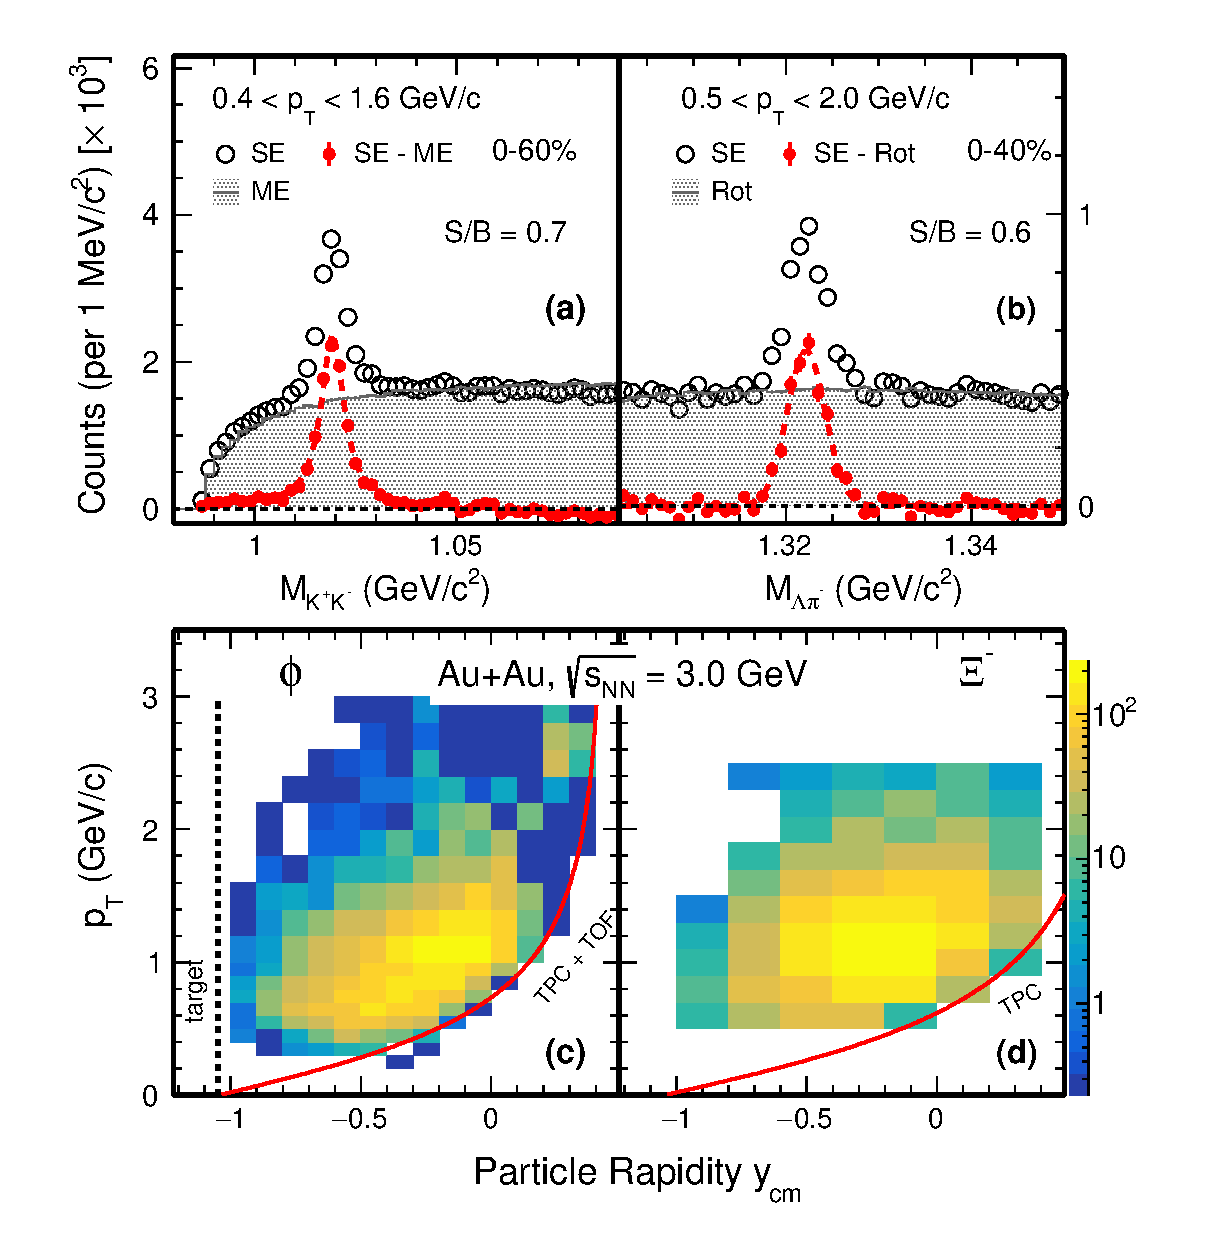
\includegraphics[width=0.50\textwidth]{fig1_signal.eps}
  \caption{Invariant mass distributions of $K^+K^-$ ($\Lambda\pi^-$) in the $p_T$ region of 0.4--1.6 (0.5--2.0) \,GeV/$c$ in 0--60\% (0--40\%) central Au+Au collisions at ${\sqrt{s_{\rm NN}} = \rm{3\,GeV}}$. Black open circles represent the same-event unlike-sign distribution. The grey shaded histogram represents the normalized mixed-event (rotating daughters for $\Xi^-$) unlike-sign distribution that is used to estimate the combinatorial background. The red solid circles depict the $\phi$ meson (a) and $\Xi^-$ (b) signals obtained by subtracting the combinatorial background from the same-event distribution. Reconstructed $\phi$ meson (c) and $\Xi^-$ hyperon (d) acceptance plot, $p_T$ vs. rapidity in the center-of-mass frame ($y_{\rm cm}$) in Au+Au collisions at ${\sqrt{s_{\rm NN}} = \rm{3\,GeV}}$. The dotted line indicates the target rapidity location. The red curve represents the TPC and TOF acceptance edge.}
\label{fig:phiSignal} 
\end{figure}


Figure~\ref{fig:phiSignal} (a) shows the invariant mass distribution of $K^+K^-$ pairs in the transverse momentum ($p_{T}$) region of 0.4--1.6 GeV/$c$ for 0--60\% central collisions. The combinatorial background is estimated with the mixed-event (ME) technique in which $K^+$ and $K^-$ from different events of similar characteristics (centrality, event plane angle) are paired. The mixed-event spectra are normalized to the same-event (SE) distributions in the mass range of 1.04--1.08\,GeV/$c^2$. After the subtraction of the combinatorial background, the remainder distribution is shown as red solid circles. The $K^+K^-$ invariant mass remainder distribution is fitted with a Breit-Wigner function for the signal plus a linear function which represents the remaining correlated background ($< 1\%$) from a partial reconstruction of strange hadrons. The $\phi$ meson raw yields are extracted from the Breit-Wigner function fit within the corresponding 3$\sigma$ mass window. The extracted $\phi$ signal shape is consistent with its intrinsic properties convoluted with the detector smearing effect due to finite momentum resolution ($<3\%$ for single track).
Figure~\ref{fig:phiSignal} (b) shows the invariant mass distribution of $\Lambda(p\pi^-)\pi^-$ in the $p_{T}$ region of 0.5--2.0 GeV/$c$ for $\textup{0--40\%}$ central collisions. The combinatorial background is estimated with the rotating daughter (Rot) method, in which a daughter track of $\Xi^-$ is rotated by a random angle between 150 to 210 degrees in the transverse plane. The rotated spectra are normalized to the same-event distributions in the mass ranges of 1.30--1.31 and 1.34--1.35\,GeV/$c^2$. After the combinatorial background is subtracted, the $\Lambda\pi^-$ invariant mass distributions are fitted with a Gaussian for the signal plus a linear function for the remaining correlated background. The $\Xi^-$ raw yields are obtained via histogram bin counting from the invariant mass distributions with all background subtracted within mass windows of 3$\sigma$. The reconstructed $\phi$ and $\Xi^-$ acceptances ($p_T$ vs. $y_{cm}$) in the collision center-of-mass frame are shown in Fig.~\ref{fig:phiSignal} (c) and (d), respectively.
The target is located at $y_{cm} = -1.05$, using the convention where the beam travels in the positive direction. The red curve represents the TPC and TOF acceptance edge. The reconstructed $\phi$ and $\Xi$ in this analysis cover the range from the target to mid-rapidity.

%The reconstructed $K^-$, $\phi$, and $\Xi^-$ 
Particle
raw yields are calculated in each centrality and $p_{T}$ bin within each rapidity slice. 
The raw yields are corrected for the TPC acceptance and tracking efficiency, %$\varepsilon_{\rm TPC}$, 
the particle identification efficiency, %$\varepsilon_{\rm PID}$ 
and the TOF matching and PID efficiency. The final average reconstruction (including acceptance etc.) efficiency is $\sim$0.30, 0.04, and 0.02 for $K^-$, $\phi$ and $\Xi^-$, respectively.

\begin{figure}
\centering
\hspace*{-4mm}
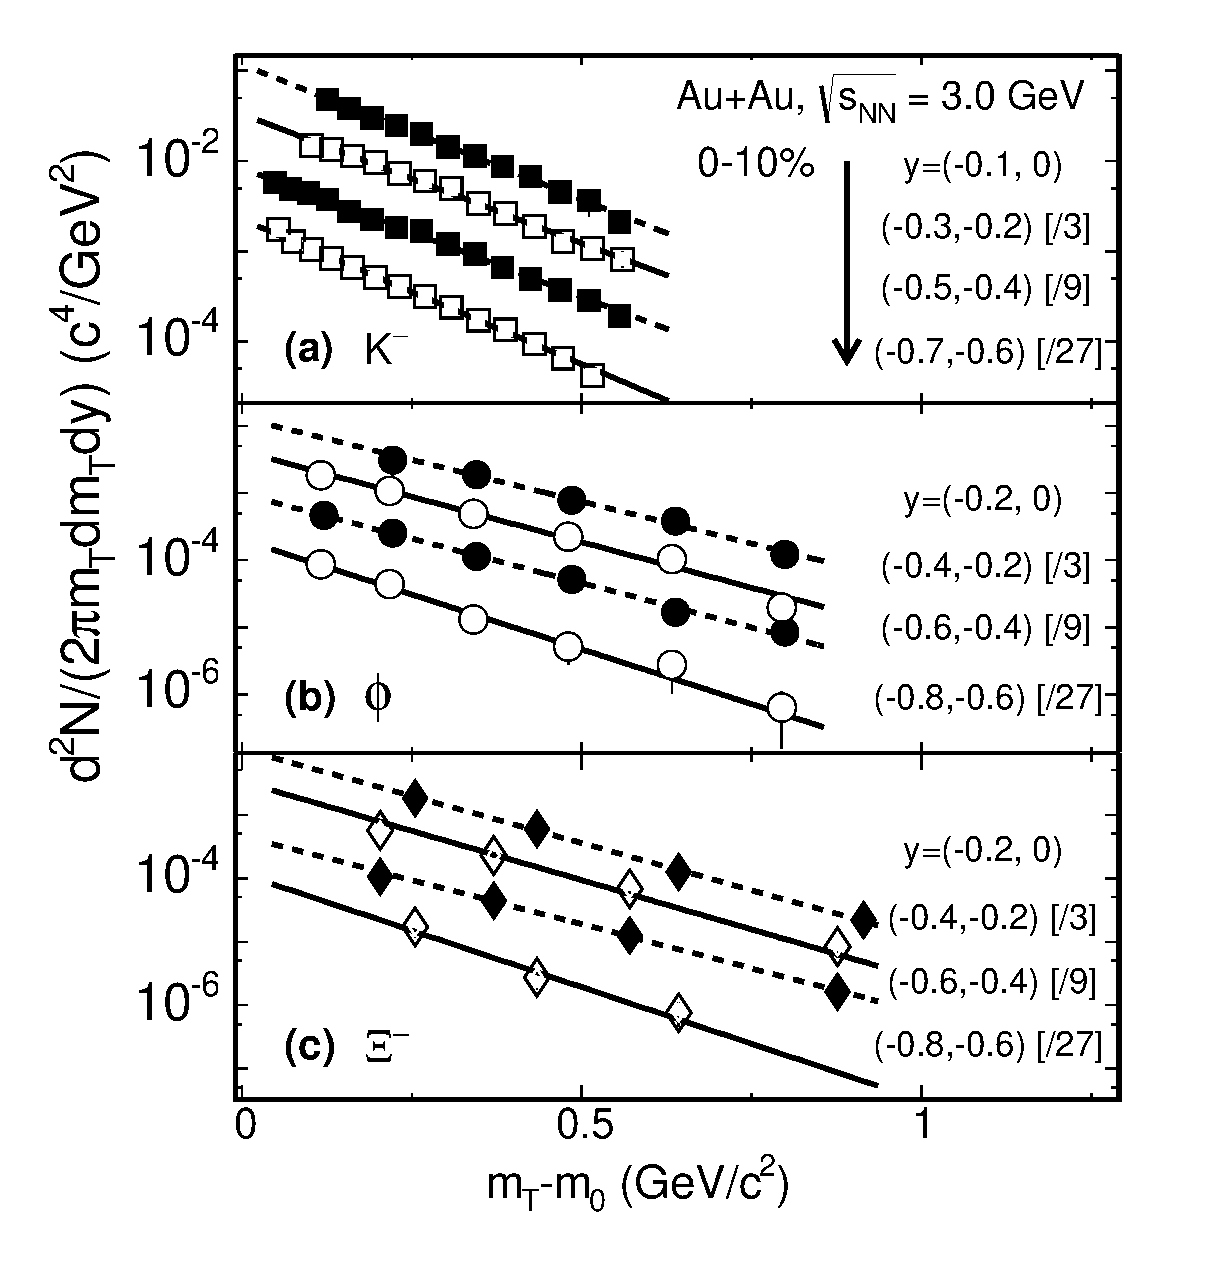
\includegraphics[width=0.43\textwidth]{fig2_mT_spectra.eps}
  \caption{$K^-$ (a), $\phi$ meson (b) and $\Xi^-$ (c) invariant yields as a function of $m_T-m_0$ for various rapidity regions in 0--10\% central Au+Au collisions at ${\sqrt{s_{\rm NN}} = \rm{3\,GeV}}$. Statistical and systematic uncertainties are added quadratically here for plotting. Solid and dashed black lines depict $m_T$ exponential function fits to the measured data points with scaling factors in each rapidity windows.}
\label{fig:phimTSpectra} 
\end{figure}

The systematic uncertainty of the raw yield extraction is estimated by changing the histogram fitting method to bin counting method or by changing the fitting ranges. The maximum difference between these scenarios and the default one is considered as one standard deviation. The contribution varies by $p_T$, rapidity, and centrality and the overall contribution is less than 5\% for the invariant yield. The systematic uncertainty in the TPC acceptance and efficiency correction $\varepsilon_{\rm TPC}$ is estimated by varying the cuts on track selection criteria and topological variables (for $\Xi^-$ only). The contribution to the total yield is about 4-5\% for $K^-$, 13-16\% for $\phi$ and 6-10\% for $\Xi^-$. This leads to a 10-13\% (12-18\%) uncertainty in the measured $\phi/K^-$ ($\phi/\Xi^-$) ratio. The uncertainty of the PID efficiency correction is estimated in a similar way by varying the PID selection cuts and the contribution is less than 3\% to the total yield.
For the $p_T$ integrated yield, one important source of systematic uncertainty comes from the extrapolation to the full $p_T$ range due to the limited acceptance. This is estimated by choosing several fitting functions~\cite{STAR_particleYield}. The maximum difference between these scenarios and the default one ($m_T$-exponential) is quoted as one standard deviation from this source. This contribution is 5-7\% for $K^-$, 14-17\% for $\phi$ and 13-15\% for $\Xi^-$. As a cross-check, we conducted the measurement of $\Xi^{-}$ lifetime from the same data and the result, $164.2\pm6.6$ ps is consistent with the PDG value, $163.9\pm1.5$ ps. The corrected $p_T$ spectra are symmetry consistent with respect of y=0 between positive and negative rapidity for the covered $p_T$ range.


\begin{table*}
\centering{
  \caption{$\phi$, $K^-$, $\Xi^-$ integrated yields and $\phi/K^-$ and $\phi/\Xi^-$ ratios for given centrality classes in Au+Au collisions at ${\sqrt{s_{\rm NN}} = \rm{3\,GeV}}$. The first error given corresponds to the statistical one, the second to the systematic error.}
\begin{tabular}{c|c|c|c|c|c} \hline \hline
  Centrality & $\phi$ $(10^{-3})$  & $K^-$ $(10^{-2})$ & $\phi/K^-$ & $\Xi^-$ $(10^{-3})$ & $\phi/\Xi^-$  \\ \hline
  ~~~0--10\%~~~   & ~~$20.1\pm1.4\pm3.8$~~  & ~~$8.70\pm0.02\pm 0.53$~~  & ~~$0.231\pm0.016\pm0.042$~~ & ~~$13.9\pm0.8\pm2.4$~~ & ~~$1.45\pm0.13\pm0.34$~~ \\
  10--40\%  & $8.5\pm0.4\pm1.7$  & $3.39\pm0.01\pm 0.20$  & $0.249\pm0.011\pm0.046$ & $3.61\pm0.32\pm0.59$ & $2.34\pm0.23\pm0.65$ \\
  40--60\%  & $2.6\pm0.2\pm0.5$  & $0.79\pm0.01\pm 0.06$  & $0.327\pm0.029\pm0.069$ & --- & --- \\ \hline
\end{tabular}
\label{table:yieldTratio}
}
\end{table*}

\begin{figure}
\centering
\hspace*{-4mm}
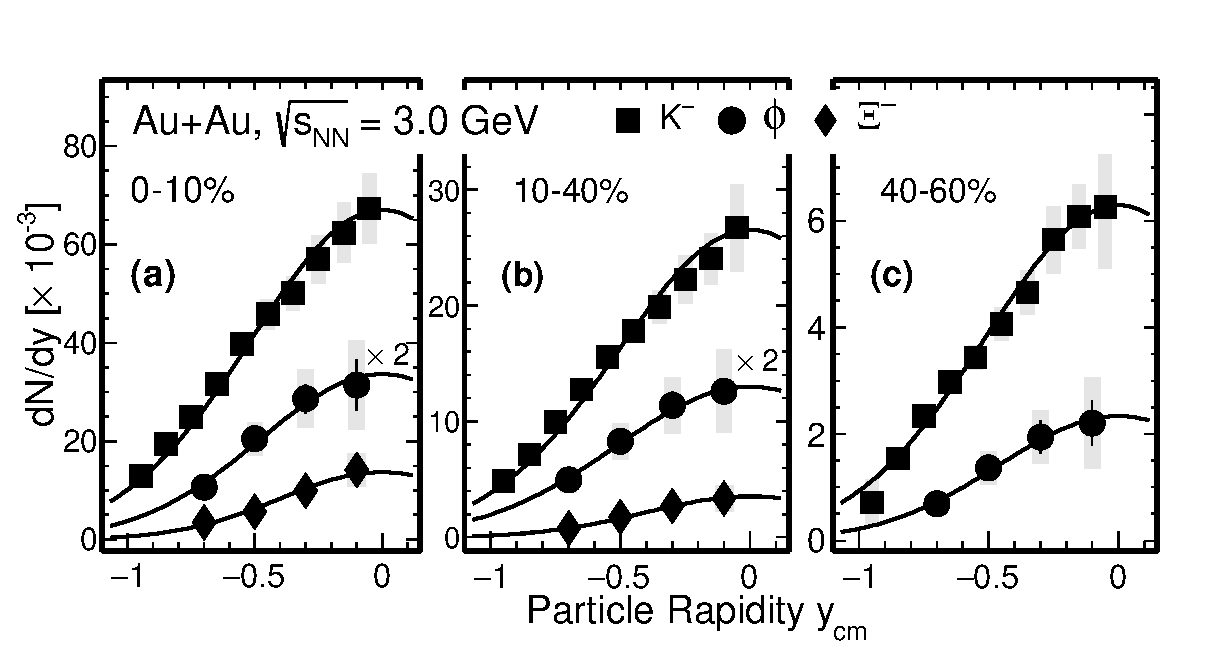
\includegraphics[width=0.5\textwidth]{fig3_dndy.eps}
  \caption{Rapidity density distributions of $K^-$ (squares), $\phi$ meson (circles) and $\Xi^-$ (diamonds) $p_T$-integrated yields $dN/dy$ in 0--10\% (a), 10--40\% (b) and 40--60\% central (c) Au+Au collisions at ${\sqrt{s_{\rm NN}} = \rm{3\,GeV}}$. %The full symbols show the measured data, while the open ones are data reflected with respect to $y=0$ in the center-of-mass frame. 
  Solid lines depict Gaussian function fits to the data points.}
\label{fig:phiYSpectra} 
\end{figure}

Figure~\ref{fig:phimTSpectra} shows the acceptance $\times$ efficiency corrected $K^-$, $\phi$ meson and $\Xi^-$ invariant yields as a function of $m_T-m_0$ ($m_T = \sqrt{m_{0}^{2}+p_{T}^2}$) for various rapidity ranges in 0--10\% central Au+Au collisions at ${\sqrt{s_{\rm NN}} = \rm{3\,GeV}}$. %The $\phi$-meson, $K^-$ and $\Xi^-$ spectra in some rapidity intervals are scaled with arbitrary factors indicated in the figure for clarity. 
Dashed and solid lines depict fits to the spectra with the $m_T$-exponential function in order to extrapolate the unmeasured $p_T$ ranges. 
The $p_T$ integrated rapidity distributions $dN/dy$ are displayed in Fig.~\ref{fig:phiYSpectra} for Au+Au collisions at ${\sqrt{s_{\rm NN}} = \rm{3\,GeV}}$ for three different centralities. %The full symbols show the measured data, while the open ones are data reflected with respect to $y=0$ in the center-of-mass frame. 
Solid curves depict Gaussian function fits to the data points with the centroid parameter fixed to zero. They are used to extrapolate to the unmeasured rapidity region in order to calculate the total multiplicities per triggered event for each particle.


\begin{figure}
\centering
\hspace*{-4mm}
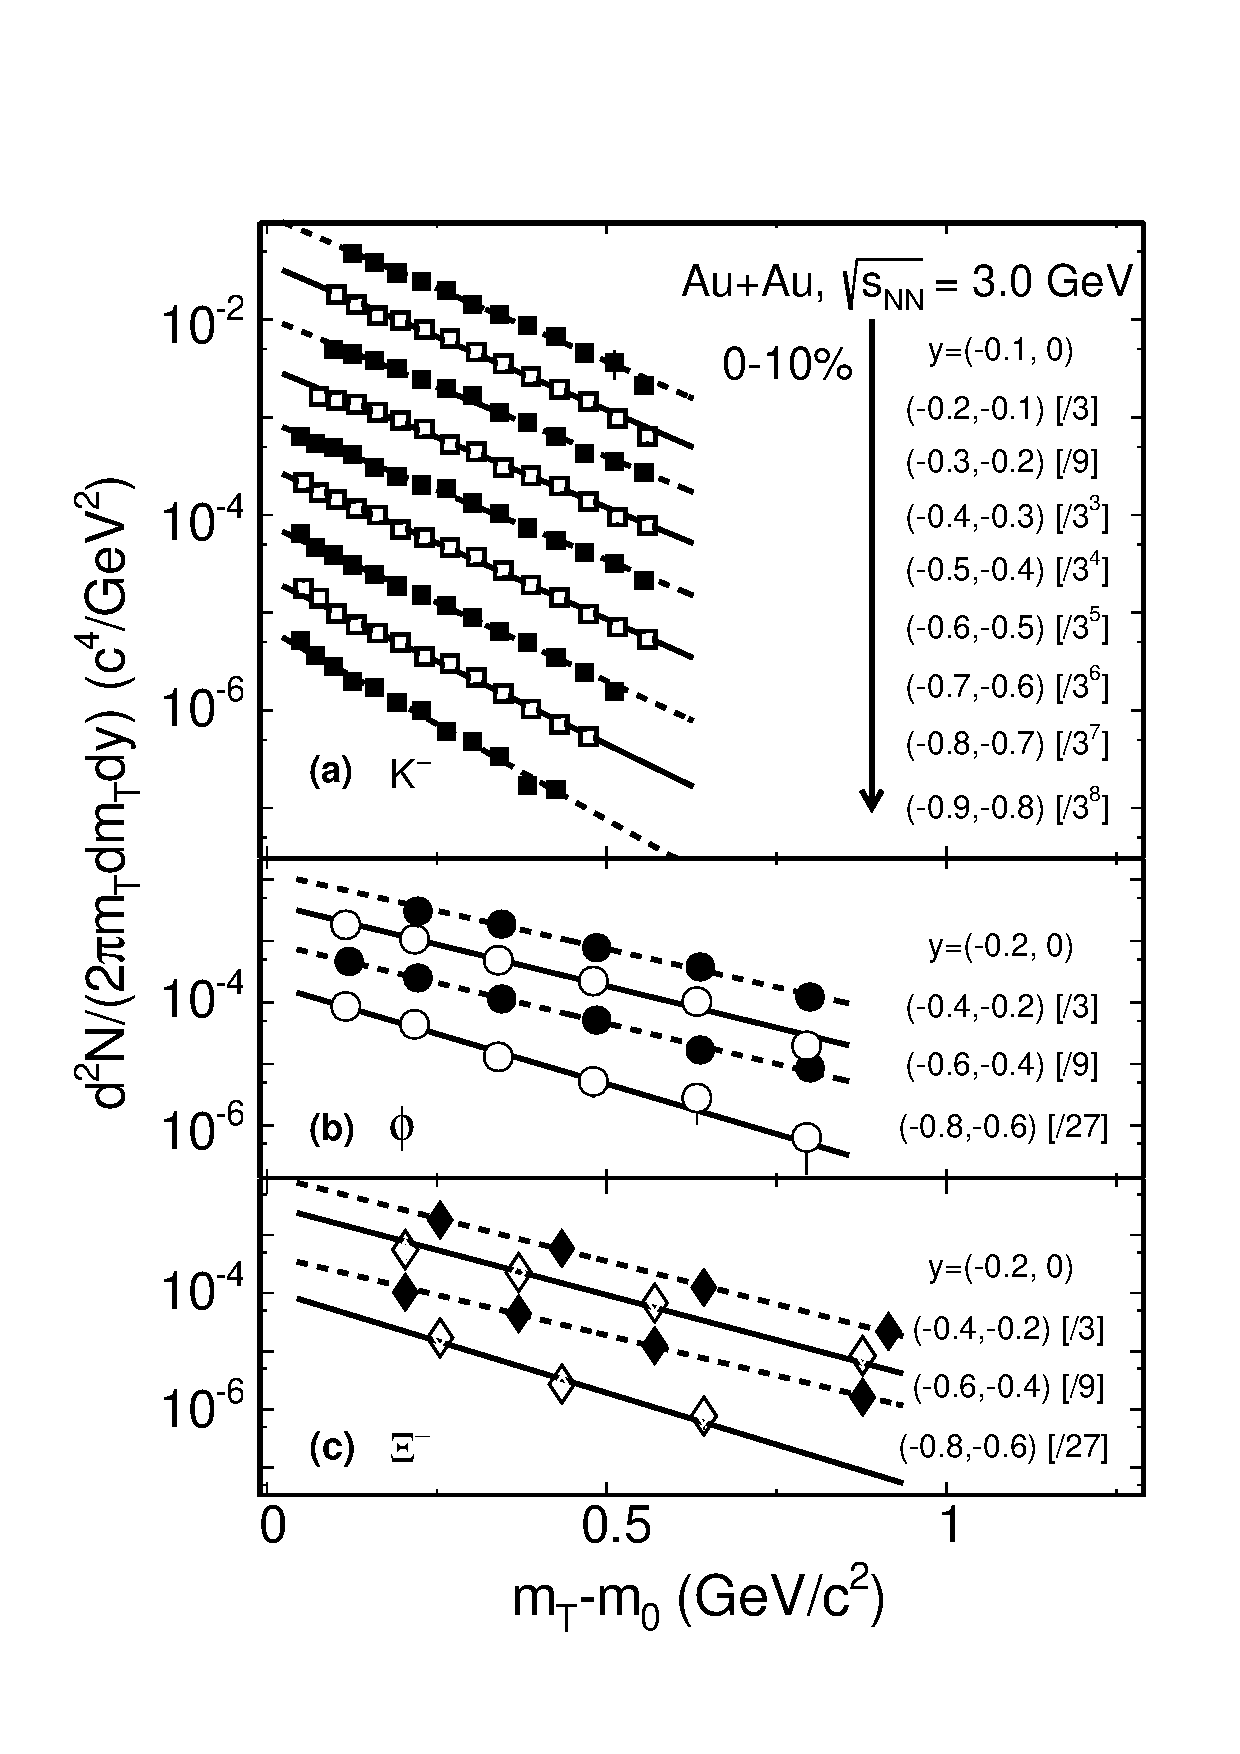
\includegraphics[width=0.38\textwidth]{fig4_phi_over_kminus_zoomin.pdf}
  \caption{$\phi/K^-$ (a) and $\phi/\Xi^-$ (b) ratio as a function of collision energy, $\sqrt{s_{\rm NN}}$. The solid black circles show the measurements presented here in 0-10\% centrality bin, while empty markers in black are used for data from various other energies and/or collision systems~\cite{E917_phi,NA49_phi,FOPI_phi_AlAl,FOPI_phi_NiNi,HADES_phi_ArKCl,HADES_phi_AuAu,Xi_ArKCl_HADES,star_bes_strangeness}. The vertical grey bands on the data points represent the systematic uncertainties. The grey solid line represents a THERMUS calculation based on the Grand Canonical Ensemble (GCE) while the dotted lines depict calculations based on the Canonical Ensemble (CE) with different values of the strangeness correlation radius ($r_c$)~\cite{THERMUS_WHEATON200984,Andronic_2018Naure}. The green dashed line, green shaded band and the solid red line show transport model calculations from the public versions $\textup{UrQMD}^{1}$~\cite{urQMD,UrQMD_2}, modified $\textup{UrQMD}^{2}$~\cite{Steinheimer_2015_UrQMD} and SMASH~\cite{Elfner_SMASH}, respectively.}
\label{fig:phi2Kratio} 
\end{figure}


The $\phi/K^-$ and $\phi/\Xi^-$ ratios are presented in Fig.~\ref{fig:phi2Kratio} as a function of collision energy $\sqrt{s_{\rm NN}}$, including the midrapidity data in central Au+Au or Pb+Pb data from the AGS, SPS and RHIC BES at higher energies and $4\pi$\,acceptance data from SIS at lower energies. The black solid circles show our measurements in 0-10\% centrality bin in Au+Au collisions at ${\sqrt{s_{\rm NN}} = \rm{3\,GeV}}$. The measured $\phi$, $K^-$ and $\Xi^-$ yields in 4$\pi$ and the $\phi/K^-$, $\phi/\Xi^-$ ratios in different centrality bins are listed in Tab.~\ref{table:yieldTratio}. The $\phi/K^-$ and $\phi/\Xi^-$ ratios measured at 3\,GeV are %significantly ($5\sigma$) above the GCE prediction ($\sim$0), and 
slightly higher than the values at high energies for $\sqrt{s_{\rm NN}}\geqslant$ 5\,GeV~\cite{NA49_phi,NA49_piK,NA49_piK2,NA49_Xi,E917_phi,ALICE_phi_2p7TeV,STAR_phi_64a200GeV,Xi_ArKCl_HADES,star_bes_strangeness} despite the collision energy being very close to the $\phi$ threshold and below the $\Xi^-$ threshold in NN collisions. %The measured data points follow the energy dependence trend, with the value gradually increasing with decreasing energy at low $\sqrt{s_{\rm NN}}$. %Our measured data points confirmed this enhancement observation which limited by the precision in the previous measurements.

Various curves in Fig.~\ref{fig:phi2Kratio} represent the predictions of $\phi/K^-$ and $\phi/\Xi^-$ ratios from several model calculations in central A+A collisions. Statistical model calculations, based on the Grand Canonical Ensemble and Canonical Ensemble for strangeness with several different choices of strangeness correlation length ($r_c$), were calculated using the $\textup{THERMUS}$ package~\cite{THERMUS_WHEATON200984} with energy dependent freeze-out parameters ($T_{\rm ch}$, $\mu_B$) taken from~\cite{Andronic_2018Naure}. These parameters were extracted through a thermal model fit to the particle yields at mid-rapidity. We noted that the calculated ratios from GCE have some dependence on the choice of $\mu_{S}$ and in this calculation, $\mu_{S}$ was chosen to be $\mu_{B}/4$ based on the extracted parameters in STAR BES-I data~\cite{star_bes_strangeness}. The strangeness number is conserved on average in the GCE. The GCE calculation fails to describe our new measurements at ${\sqrt{s_{\rm NN}} = \rm{3\,GeV}}$ (5.2$\sigma$ deviation), which indicates the thermal particle phase-space at low energies is far from the GCE limit and the local treatment of strangeness conservation is crucial~\cite{BraunMunzinger:2003zd}. In the canonical approach, the correlation length, $r_c$, defines a region of the particle production phase space inside which the production of the strangeness is canonically conserved. Both the $\phi/K^-$ and $\phi/\Xi^-$ data from our measurement favor the CE thermodynamics for strangeness with a small strangeness correlation length ($r_c \leq 4.2$\,fm). It is worthwhile to point out that the CE calculations with the same $r_c$ parameter cannot describe our $\phi/K^-$ and $\phi/\Xi^-$ data simultaneously (as also observed in lighter systems and at lower collision energy ~\cite{HADES_phi_ArKCl}). The production yields of $\phi$ and $\Xi^-$ in near/sub-threshold regions based on the thermal model calculations are sensitive to the freeze-out parameters. 
A global thermal model fit with all the particle yields at 3\,GeV will help to precisely determine these thermal parameters in the future.

Previous measurements from smaller collision systems (Ar+KCl and Al+Al collisions) showed comparable or higher $\phi/K^-$ and/or $\phi/\Xi^-$ ratios at energies below 3 GeV. The previous measurement in $p$+$p$ collisions at $\textup{2.7 GeV}$ shows that $\phi/K^- = 1.04\pm0.23$ ~\cite{ANKE_phi}. The measurement in $p$+$p$ collisions at $\textup{17.3 GeV}$ shows that $\phi/K^- = 0.11\pm0.01$, comparable to that in central Au+Au/Pb+Pb collisions, while $\phi/\Xi^- = 5.09\pm0.36$, significantly larger than that in central Au+Au/Pb+Pb collisions ~\cite{NA61SHINE_pp_piKp,NA61SHINE_pp_phi,NA61SHINE_pp_Xi}. In our measurement at 3 GeV, there is no obvious difference in the $\phi/K^-$ ratio between the \textup{0--10\%} and \textup{10--40\%} central bins, while the result in the most peripheral 40--60\% central bin shows a hint of a larger value, as shown in Tab.~\ref{table:yieldTratio}. Similarly, the $\phi/\Xi^-$ ratio in mid-central collisions seems to be larger than that in central collisions. Overall, these observations are qualitatively consistent with the expectation that a smaller canonical volume in the smaller system leads to a higher observed $\phi/K^-$ and/or $\phi/\Xi^-$ ratio.

Hadronic transport models are widely used in the high baryon density region to study the properties of the produced dense matter~\cite{urQMD,UrQMD_2,Steinheimer_2015_UrQMD,Elfner_SMASH,Hartnack:2011cn,Song:2020clw}. In the modified version of the Ultra-relativistic Quantum Molecular Dynamics (UrQMD) model~\cite{Steinheimer_2015_UrQMD}, new decay channels from high mass baryon resonances to $\phi$ and $\Xi^-$ are deployed. The relevant decay branching fraction was determined by fitting the experimental data from $p$+$p$ collisions~\cite{ANKE_phi}. From the comparison shown in Fig.~\ref{fig:phi2Kratio}, the modified $\textup{UrQMD}^{2}$ calculation for central ($\rm{b}<5\,\rm{fm}$) Au+Au collisions agrees with the data points at low ${\sqrt{s_{\rm NN}}}$, including our new measurement for $\phi/K^-$.
%, while the calculation for $\phi/\Xi^-$ currently is not available in this energy. 
However calculations from the public $\textup{UrQMD}^{1}$ model underestimate our measurements for both $\phi/K^-$ and $\phi/\Xi^-$.   
%while clearly underestimating the measurements at high $\sqrt{s_{\rm NN}}\geqslant$ 5\,GeV.
Another hadronic transport approach called Simulating Many Accelerated Strongly-interacting Hadrons (SMASH) attempts to incorporate the newest available experimental data from both elementary hadronic cross sections and dilepton invariant mass spectra to constrain the resonance branching ratios~\cite{Elfner_SMASH}. The $\phi/K^-$ ratio is reasonably reproduced using SMASH in the smaller system and ${\sqrt{s_{\rm NN}}}$ below $\textup{3 GeV}$, despite the overestimation of each individual ($\phi$, $K^-$) transverse mass spectrum measured, e.g. in Au+Au $\textup{0-40\%}$ system by HADES~\cite{Elfner_SMASH,HADES_phi_AuAu}. The predicted $\phi/K^-$ ratio from the same model is about is 2.5$\sigma$ higher than central Au+Au 0-10\% collisions at $\textup{3 GeV}$. This indicates that some important in-medium mechanism for strangeness production and propagation may be missing for the large system in SMASH.


In summary, we report the first multi-differential measurement of $K^-$, $\phi(1020)$ and $\Xi^{-}$ production yields  and the $\phi/K^-$, $\phi/\Xi^-$ ratios in Au+Au collisions at ${\sqrt{s_{\rm NN}} = \rm{3\,GeV}}$ with the STAR experiment at RHIC. The measured $\phi/K^-$ ratio is $5.2\sigma$ larger than the statistical model prediction limit based on the Grand Canonical Ensemble in $\textup{0--10\%}$ central collisions. Both the results of $\phi/K^-$ and $\phi/\Xi^-$ ratios favor the model with the Canonical Ensemble treatment for strangeness and a small strangeness correlation length parameter, $r_c$, in $\textup{0--10\%}$ central Au+Au collisions. The transport models including the resonance decays can reasonably describe both our measured $\phi/K^-$ ratio at this energy and the trend of $\phi/\Xi^-$ at lower energies. Our results suggest a significant change in the strangeness production at ${\sqrt{s_{\rm NN}} = \rm{3\,GeV}}$ compared to higher collision energies, providing new insights towards the understanding of the QCD medium properties at high baryon density region~\cite{KO_sQM17}. 


% Chapter acknowledgement
%\section{Acknowledgement}
%\label{acknowledgement}

We would like to thank K. Redlich and J. Steinheimer for fruitful discussions.
We thank the RHIC Operations Group and RCF at BNL, the NERSC Center at LBNL, and the Open Science Grid consortium for providing resources and support.  This work was supported in part by the Office of Nuclear Physics within the U.S. DOE Office of Science, the U.S. National Science Foundation, the Ministry of Education and Science of the Russian Federation, National Natural Science Foundation of China, Chinese Academy of Science, the Ministry of Science and Technology of China and the Chinese Ministry of Education, the Higher Education Sprout Project by Ministry of Education at NCKU, the National Research Foundation of Korea, Czech Science Foundation and Ministry of Education, Youth and Sports of the Czech Republic, Hungarian National Research, Development and Innovation Office, New National Excellency Programme of the Hungarian Ministry of Human Capacities, Department of Atomic Energy and Department of Science and Technology of the Government of India, the National Science Centre of Poland, the Ministry  of Science, Education and Sports of the Republic of Croatia, RosAtom of Russia and German Bundesministerium f\"ur Bildung, Wissenschaft, Forschung and Technologie (BMBF), Helmholtz Association, Ministry of Education, Culture, Sports, Science, and Technology (MEXT) and Japan Society for the Promotion of Science (JSPS).

\bibliography{phi3GeV.bib}


\newpage

\vspace{5.0cm}


\section{supplemental material}

\subsection{Full Corrected $m_T$ Spectra}

Figure 5 shows the corrected $K^-$, $\phi$ meson and $\Xi^-$ invariant yields as a function of $m_T-m_0$ for various rapidity ranges in 0--10\% (left) and 10--40\% (right) centrality Au+Au collisions at ${\sqrt{s_{\rm NN}} = \rm{3\,GeV}}$. The $K^-$, $\phi$-meson and $\Xi^-$ spectra in some rapidity intervals are scaled with arbitrary factors indicated in the figure for clarity. Dashed and solid lines depict fits to the spectra with the $m_T$-exponential function in order to extrapolate the unmeasured $p_T$ ranges. Figure 6 shows the similar plot for $K^-$ and $\phi$ meson in 40--60\% centrality Au+Au collisions.

\begin{figure*}
\centering
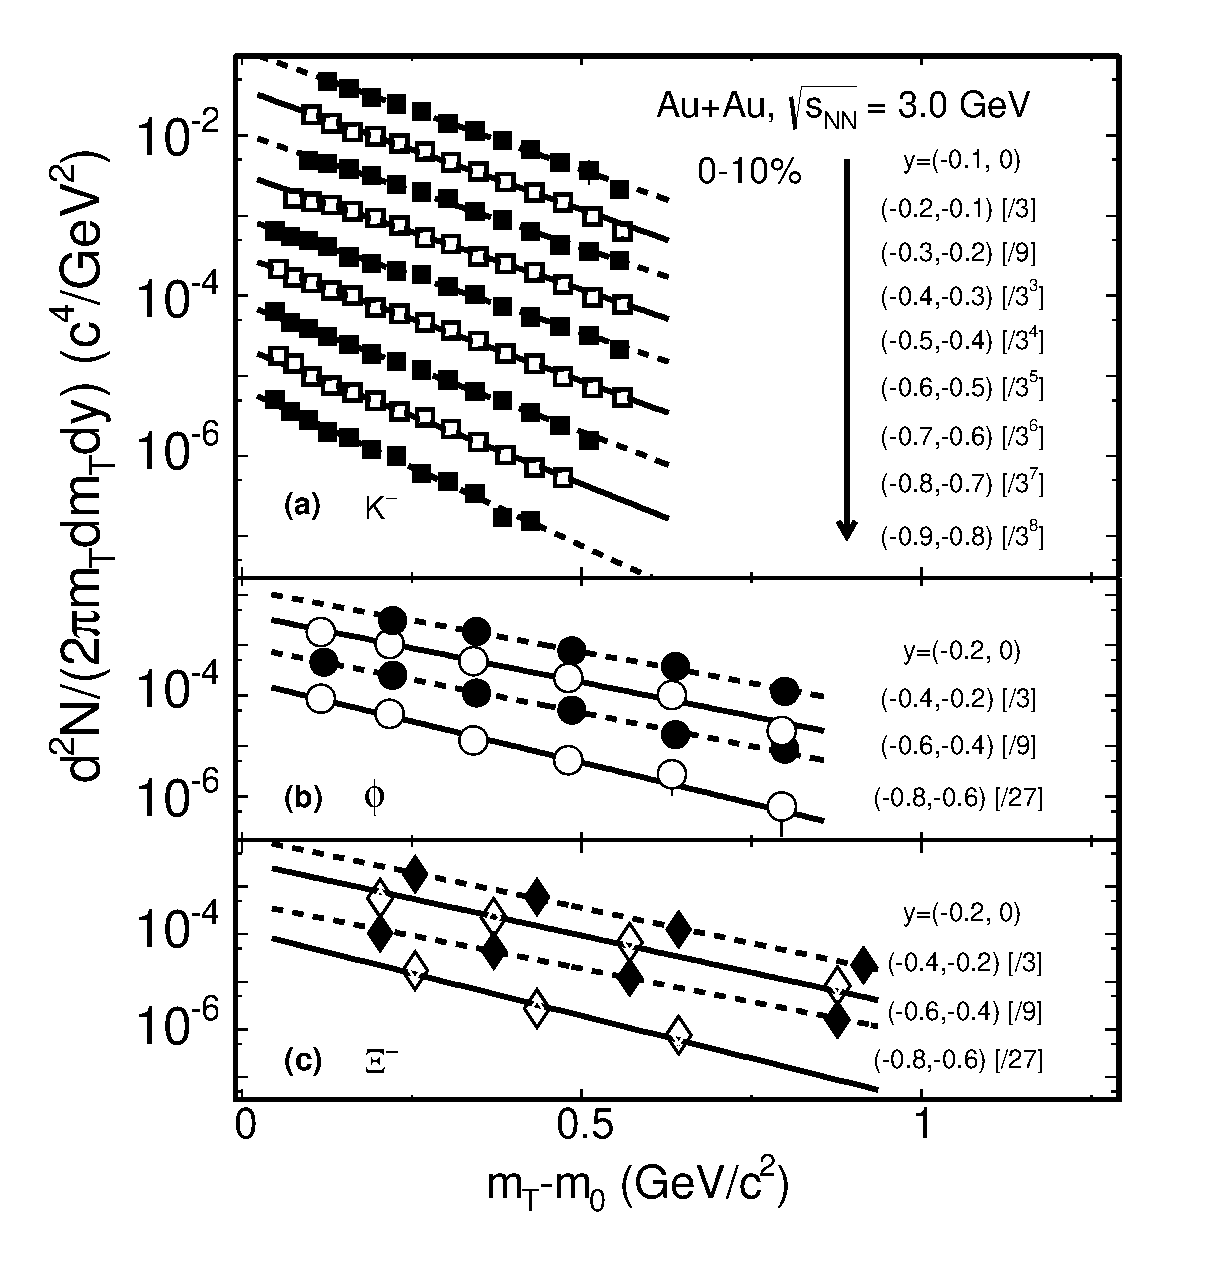
\includegraphics[width=0.43\textwidth]{fig21.eps}
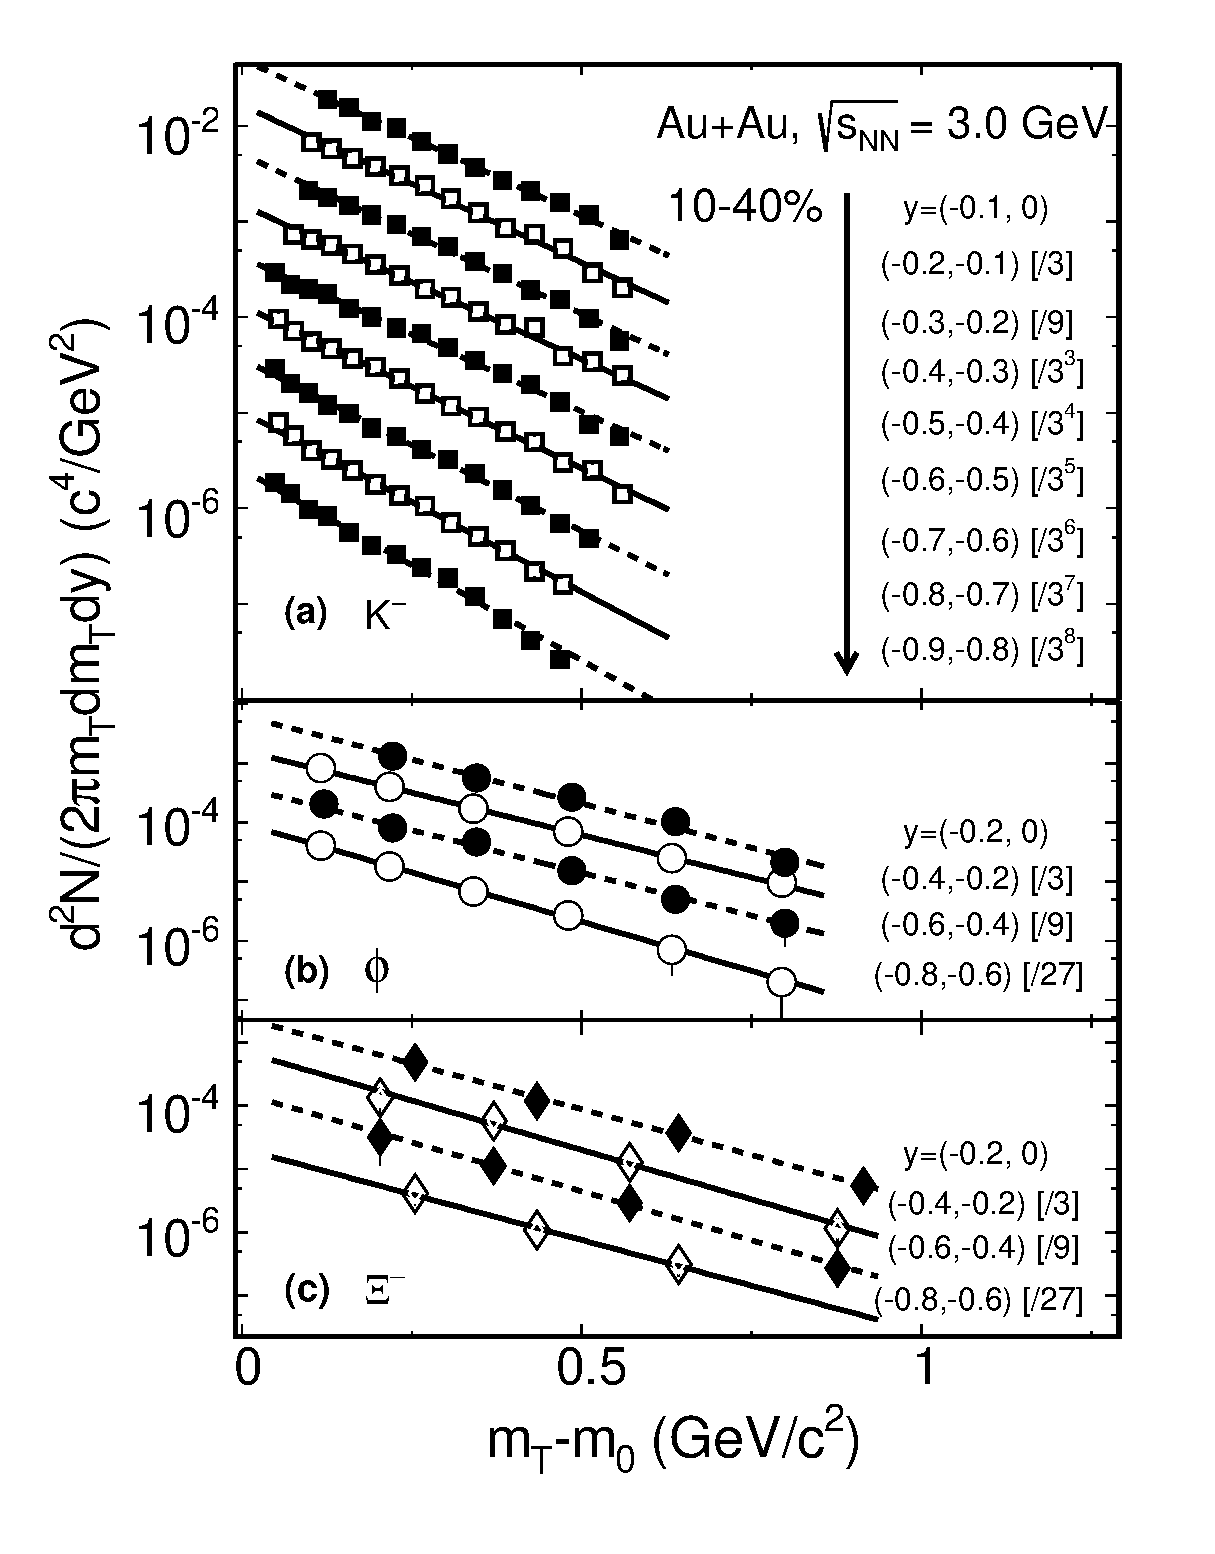
\includegraphics[width=0.43\textwidth]{fig22.eps}
\caption{$K^-$ (a), $\phi$ meson (b) and $\Xi^-$ (c) invariant yields as a function of $m_T-m_0$ for various rapidity regions in 0--10\% (left) and  10--40\% (right) centrality Au+Au collisions at ${\sqrt{s_{\rm NN}} = \rm{3\,GeV}}$. Statistical and systematic uncertainties are added quadratically here for plotting. Solid and dashed black lines depict $m_T$ exponential function fits to the measured data points with scaling factors in each rapidity windows.}
\label{fig:phimTSpectra21}
\end{figure*}

\begin{figure}
\centering
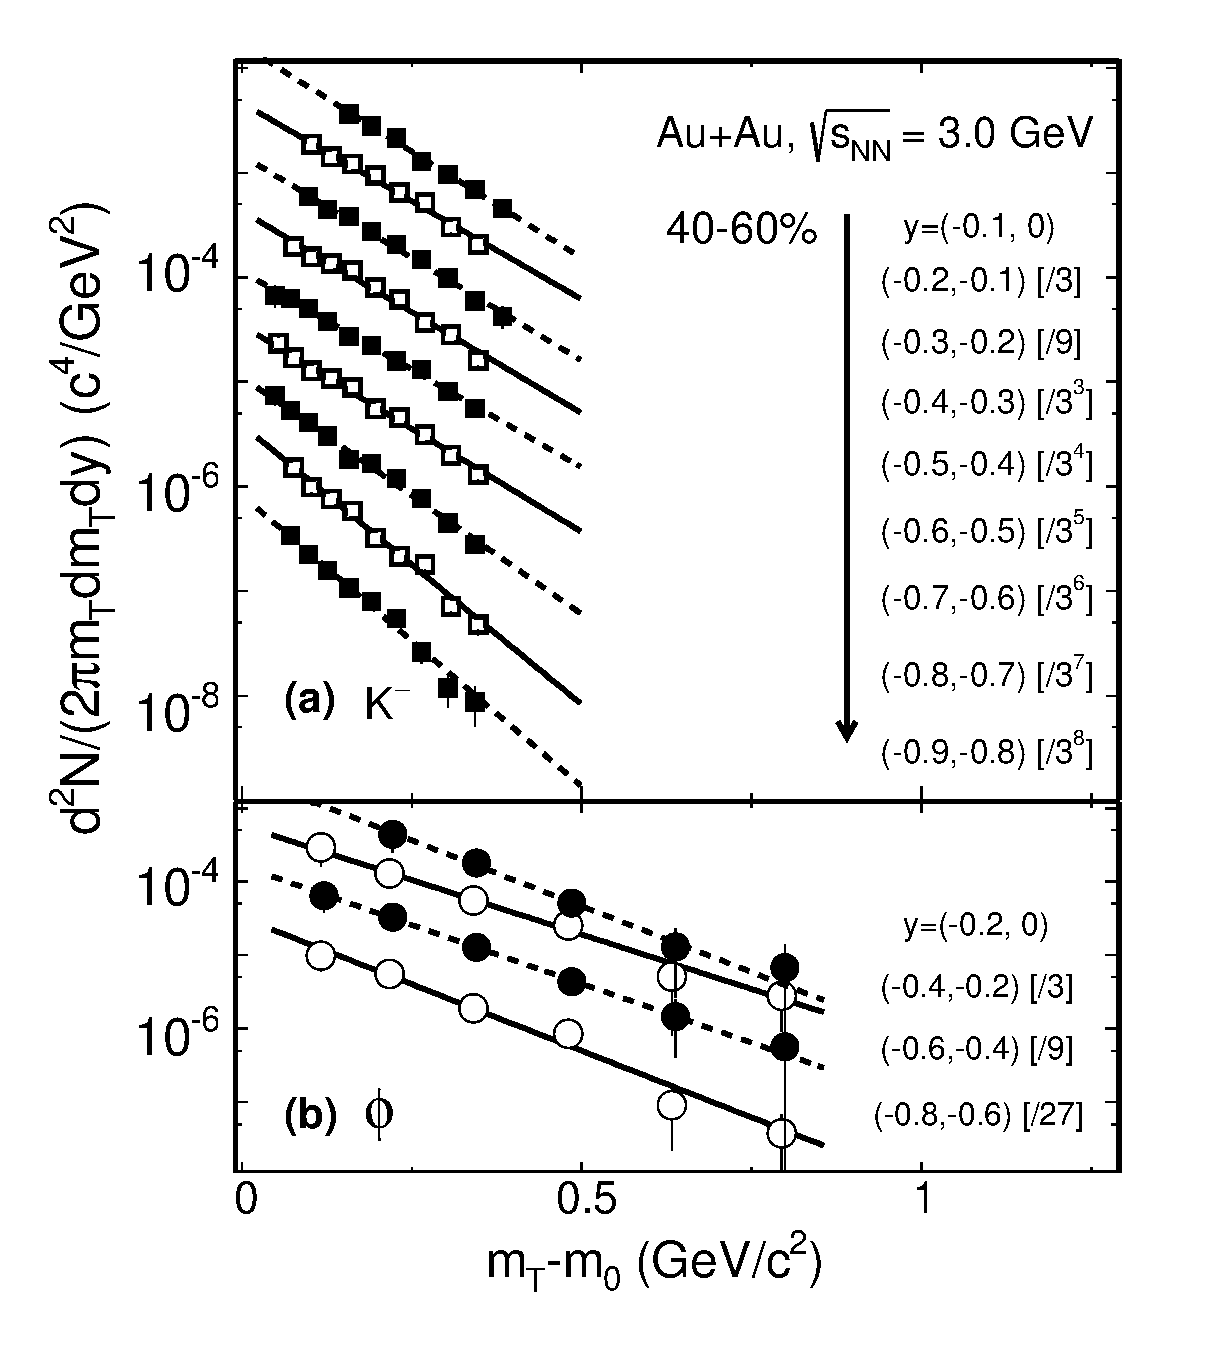
\includegraphics[width=0.43\textwidth]{fig23.eps}
\caption{$K^-$ (a) and $\phi$ meson (b) invariant yields as a function of $m_T-m_0$ for various rapidity regions in 40--60\% centrality Au+Au collisions at ${\sqrt{s_{\rm NN}} = \rm{3\,GeV}}$.}
\label{fig:phimTSpectra23}
\end{figure}


\end{document}
%
% ****** End of file apssamp.tex ******
